\chapter{Machine learning based approach}


%====================================================================================================
\section{Concepts in machine learning}
\FloatBarrier
Aim of this section is to define what exactly is understood by a term machine learning as well
as to introduce basic concepts that are common for all machine learning applications

%----------------------------------------------------------------------------------------------------
\subsection{Differences between knowledge and data based models}
\FloatBarrier
While creating a model of physical processes one of two approaches may be used.
First, is the knowledge-driven model that as the name implies relays on knowledge of underlying
laws of physics that govern the process.
The main advantage of this approach is its high explainability and reliability as every parameter
of the model corresponds with some specific physical property.
However this model has a very significant downside, it requires detailed knowledge of physical
phenomena. This means that for complex processes it might be very difficult or even
impossible, at a~given moment, to create a model. Another drawback is that the complexity of
the process grows the computational cost of its model.
If those problem makes creating usable knowledge-based model impossible or economically
non efficient a data-driven approach may be used.
It model used is chosen arbitrarily with little or no relation to underlying physics,
then model parameters are adjusted until it will fit experimental data to the best of its
capability.
The main advantage of a data-driven approach is the lack of required knowledge on process 
inner workings, which allow prediction of events which exact mechanics have not 
yet been discovered.
Another element characteristic in the data-driven approach, that can be either advantageous or
disadvantageous, is the lack of direct correlation between the complexity 
of the process and computational cost of the model.
This is a very welcome trait for complex processes like orbital atomic clock ensembles.
The main disadvantage in comparison with the knowledge-driven approach is its lower reliability and
explainability. This is the main reason why the data-driven approach is usually avoided in
critical implementations. Another significant downside is a requirement of a large amount of
experimental data for model adjustment which means that in many cases this approach simply
cannot be used.
The last thing that must be said about the data-driven approach is that it still requires some
amount of knowledge to work efficiently as the selection of models that will be adjusted to
data requires some assumption. For example, the use of linear regression assumes that the model
is linear.

%----------------------------------------------------------------------------------------------------
\subsection{What is a machine learning algorithm}
\FloatBarrier
Term machine learning describes subset of algorithms that adjusts parameter of other algorithms 
according to data. To provide more formal definition an algorithm can be described as a 
transformation function $\phi_{a}$ such that:
\begin{equation}
	\label{equ:algorithm_general}
	\mathcal{Y}_{a} = \phi_{a}(\mathcal{X},\Theta_{a}),
\end{equation}
where $\mathcal{Y}_{a}$ is set of algorithm responses, $\mathcal{X}$ is set of inputs 
and $\Theta_{a}$ is algorithm parameter set.
Input space $\mathcal{U}_{x}$ and response space $\mathcal{U}_{y}$ can be simply a numerical
space, in which case algorithm is called numerical algorithm, but can also represent more 
abstract concepts. For example in case of database software input space will consist of 
queries while response space will contain information stored in database as well as error 
status in case query was written incorrectly.
Machine learning algorithm, denoted as $\phi_{m}$ can also be described in that general form
however what is special in this case is that input space $\mathcal{U}_{m}$ consists of either :
\begin{equation}
	\label{equ:supervised_input}
	\mathcal{X}_{m} = \{\phi_{a}, \mathcal{X}_{a}, \mathcal{Y}_{a}, \Theta_{a} \},
\end{equation}
in case of supervised learning or just :
\begin{equation}
	\label{equ:supervised_input}
	\mathcal{X}_{m} = \{\phi_{a}, \mathcal{X}_{a}, \Theta_{a} \},
\end{equation}
in case of unsupervised learning.
In both cases response of machine learning algorithm is described as a:
\begin{equation}
	\label{equ:ml_response}
	\mathcal{Y}_{m} = \{\hat{\Theta}_{a}, E_{a}\},
\end{equation}
where $\hat{\Theta}_{a}$ is adjusted set of parameters and $E_{a}$ is value prediction 
error for this new set of parameters.
Aim of machine learning algorithm is to adjust parameters $\Theta_{a}$ of given algorithm 
$\phi_{a}$ in such a way to minimize error $E_{a}$ for given data. In case of supervised learning
a correct response $\mathcal{Y}_{a}$ for inputs is known where in case of unsupervised learning
only input set $\mathcal{X}_{a}$ is known. In order to avoid confusion parameters of machine 
learning algorithm $\Theta_{m}$ will be referred to as a \textit{metaparameters}. 
Exact set of meteaparameters vary between specific algorithms, however there is one 
crucial metaparameter that will appear in every machine learning algorithm.
That metaparameter is error function as it is required for error value calculation and as 
minimization of that value is goal of machine learning it is mandatory to be able to calculate it.

%----------------------------------------------------------------------------------------------------
\subsection{Error function}
\FloatBarrier
As an error function is used for calculation of value that will be minimized by a machine 
learning algorithm correct choice of that function is crucial decision when designing such
algorithm.
Due to scope of this work attention will be given only to error function used in supervised 
learning of numerical algorithms.
Error for single pair of predicted value $\hat{y}$ and actual value $y$ can be described as
distance between them in response space $\mathcal{U}_{y}$:
\begin{equation}
	\label{equ:dist_general}
	E = f_{DIST}(\hat{y},y),
\end{equation}
where $f_{DIST}$ is distance function, alternatively called metric.
Distance function is a function that gives a distance between each pair of point elements of a set.
If a set have a distance function defined it is called a metric space. 
In order to be classified as a metric function $f_{DIST}$ over a Cartesian square of a universe 
$\mathcal{U}$ it must display following properties:
\begin{enumerate}
	\item $f_{DIST} : \mathcal{U} \times \mathcal{U} \to \mathbb{R}^{+}$
	\item identity of indiscernibles : $f_{DIST}(x_{0}, x_{1})=0 \leftrightarrow x_{0} = x_{1}$,
	\item symmetry : $f_{DIST}(x_{0},x_{1})=f_{DIST}(x_{1},x_{0})$,
	\item triangle inequality : $f_{DIST}(x_{0},x_{1}) \leq f_{DIST}(x_{0},x_{2}) +
		f_{DIST}(x_{1},x_{2})$. 
\end{enumerate}

There are many types of metrics however within scope of this work attention will be given only to
distance functions related to $\ell$ norms.
As such error function for single prediction will be described as: 
\begin{equation}
	\label{equ:dist_norm}
	E = \Vert (\hat{y}-y) \Vert_{k},
\end{equation}
where notation $\Vert \bullet \Vert_{k}$ describes $k$ norm of given value.
Norm is a function from a real or complex vector space to the non negative real number space
that describes distance of a point from the origin.
Origin is the point for which values of all dimension are equal to zero, in case of calculating
$\ell$ norm for difference between two points subtrahend is treated as a origin point.
General equation describing a $\ell_{k}$ norm in $n$ dimensional space is:
\begin{equation}
	\label{equ:ell_norm}
	\Vert x \Vert_{k} = (\vert x_{0} \vert^{k} + \vert x_{1} \vert^{k} + \cdots +
	\vert x_{n} \vert^{k})^{1/k},
\end{equation}
where $\vert x \vert$ is an absolute value of $x$.
\begin{figure}[htb] 
	\label{fig:l_norms}
	\centering
	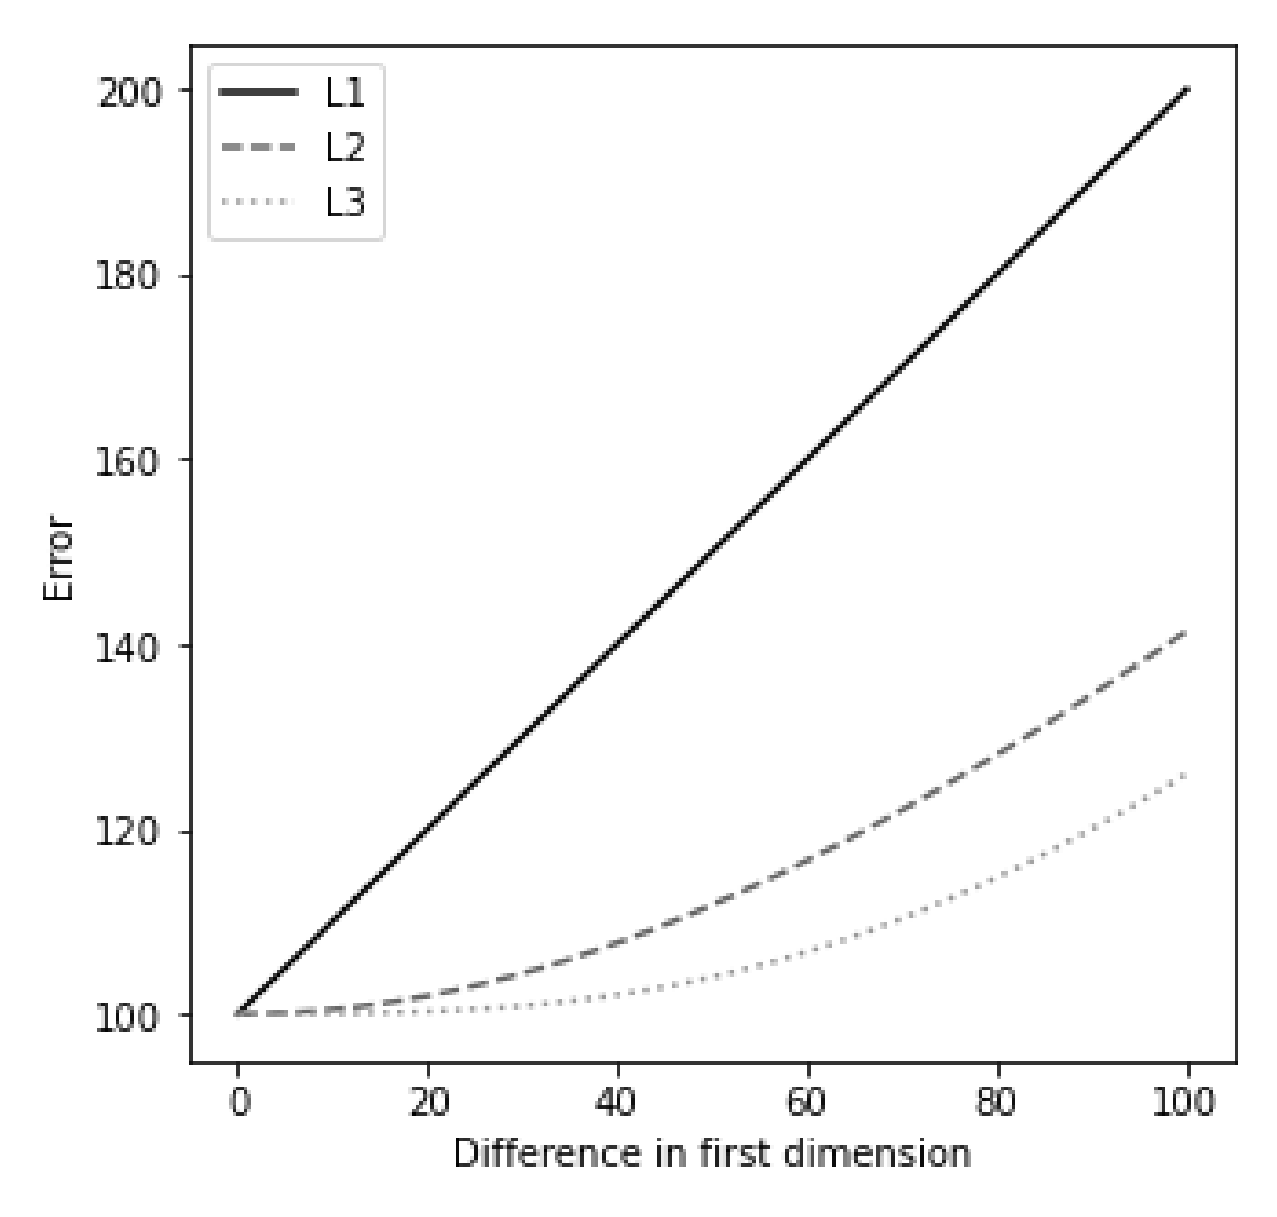
\includegraphics[width=0.5\textwidth]{figures/l_norms}
	\caption{Relation between error and difference in first dimension values with second 
	dimension difference at constant 100}
\end{figure}
\textbf{TODO: DESCRIBE WHY USE GIVEN NORMS IN MORE DETAIL}
Norms usually used in error calculation are $\ell_{1}$ and $\ell_{2}$, due to their frequent use
not only in this field they are given specific names.
Norm $\ell_{2}$ is called Euclidean norm and is equivalent to intuitive understanding of distance
while norm $\ell_{1}$ is called Manhattan distance and is related to distance between points on 
grid.
Euclidean distance is used for calculation of Root Mean Squared Error (RMSE). If we define 
knowledge base $K$ as a set of pairs $(x,y)$ where $x$ is input and $y$ an expected output
while prediction is realised by hypothesis $\hat{y} = h(x,\phi)$ error can be described as:
\begin{equation}
	\label{equ:mse}
	f_{RMSE}(K,h) = \sqrt{\frac{1}{\vert K \vert} \sum_{(x,y) \in K}(h(x,\phi)-y)^2},
\end{equation}
where $\vert K \vert$ is cardinality of knowledge base.
Manhattan distance is in turn used to calculate Mean Average Error (MAE):
\begin{equation}
	\label{equ:mae}
	f_{MAE}(K,h) = \frac{1}{\vert K \vert} \sum_{(x,y) \in K}\vert (h(x,\phi)-y)\vert.
\end{equation}
Those two error values will be used in this work.


%----------------------------------------------------------------------------------------------------
\subsection{Deep learning}
\FloatBarrier
At time when experiments described in this dissertation were conducted a new approach to 
machine learning called Deep Learning (DL) became highly popular.
Due to that popularity term deep learning is often overused and misrepresented marketing 
purposes. In this section an attempt will be made to explain what exactly constitutes as a
deep learning and describe what sort of challenges.
Term deep learning can be applied only to a subset of machine learning algorithms that have
layer based architecture, usually a neural networks.
In such implementation whole data processing algorithm can be described as a transformation:
\begin{equation}
	\label{equ:spaces1}
	\phi = \mathcal{U}_{OBS} \Rightarrow \mathcal{U}_{RES},
\end{equation}
where $\mathcal{U}_{OBS}$ is called observation space and $\mathcal{U}_{RES}$ is response space.
In case of simple single layer system observation space is directly transformed into a 
response space, however in case of multi layer model there are intermediate encoding spaces.
In such case representation spaces are numbered by index of layer which outputs them. 
So in case of $n$ layer system it would be $\{\mathcal{U}_{0}, \mathcal{U}_{1},
\cdots, \mathcal{U}_{n}\}$ where indexes $0$ and $n$ are special as 
$\mathcal{U}_{0}=\mathcal{U}_{OBS}$ and $\mathcal{U}_{n}=\mathcal{U}_{RES}$.
In that case a function transforming observation into a reaction can be described as a 
convolution of multiple encoding function.
\begin{equation}
	\label{equ:spaces_transform}
	\phi = \phi_{1} \otimes \phi_{2} \otimes \cdots \otimes \phi_{n}.
\end{equation}
Transformation $\phi_{n}$ is called output layer, while other transformation are referred to
as a hidden layers as their result is not visible during normal operation of algorithm.
Until recently almost all architectures used a single hidden layer and architectures with more
than 3 hidden layers were almost unheard of.
This is due to three issue that show up in systems with higher amount of layer: signal vanishing,
signal explosion and rise in computation due to high parameter count.


%====================================================================================================
\section{Regression approximation}
\FloatBarrier

%----------------------------------------------------------------------------------------------------
\subsection{Linear regression}
\FloatBarrier
\label{sec:linear_regression}
Linear predictor function is a linear combination of a set of coefficients and explanatory 
variables (independent variables), whose value is used to predict the outcome of a
dependent variable. Linear predictor is described as:
\begin{equation}
	\label{equ:linear_predictior}
	\hat{y} = \Theta_{0} + \Theta_{1}x_{1} + \cdots + \Theta_{n}x_{n},
\end{equation}
where $\hat{y}$ is predicted value,$n$ is feature count, $x_{i}$ is value of i-th feature
and $\Theta_{j}$ is j-th parameter.
Parameter $\Theta_{0}$ is special as it is not corresponding to any feature, that parameter
is called a \textit{bias term} or just \textit{bias}.
Predictor will return value of bias if all inputs are set to zero.
Function that allows prediction is called hypotesis function and is written as $\hat{y} = h(x)$.
With assumption that input vector for such function is $x=[1, x_{1}, \cdots, x_{n}]$ then 
a hypotesis function of a linear predictor can be defined as:
\begin{equation}
	\label{equ:linear_hyp}
	\hat{y} = h_{\Theta}(x) = \Theta^{T}\cdot x.
\end{equation}
To define how well prediction fit actuall data a error function must be selected and then one
of to approaches for minimizing it must be applied. Gradient based approach will be described 
is section \ref{sec:gradient} here a analytical approach based on a normal equation will be shown.
To derieve normal equation a MSE will be used as a error function, if other function would be 
selected a different normal equation would be a result.
In matrix notation hypothesis function can be described as :
\begin{equation}
	\label{equ:linear_hyp_matirx}
	\hat{Y} = h_{\Theta}(X) = \Theta^{T}\cdot X,
\end{equation}
where $X$ is input matrix such that each row represent single observation and each column 
single feature:
\begin{equation}
	\label{equ:input_matrix}
	X_{m\times m}=\left( \begin{array}{c c c c c}
		1& x^{(1)}_{1}& x^{(1)}_{2}& \cdots& x^{(1)}_{n}\\
		1& x^{(2)}_{1}& x^{(2)}_{2}& \cdots& x^{(2)}_{n}\\
		1& x^{(3)}_{2}& x^{(3)}_{2}& \cdots& x^{(3)}_{n}\\
		\vdots&\vdots&\vdots&\ddots&\vdots\\
		1& x^{(m)}_{2}& x^{(m)}_{3}& \cdots& x^{(m)}_{n}\\
	\end{array}\right),
\end{equation}
where $x^{(i)}_{j}$ denotes value of $j$ feature of $i$ observation.
Using this definitions the least-squares error function can be represented in matrix form as:
\begin{equation}
	\label{equ:mse_matrix}
	f_{MSE}(X,y) = \frac{1}{2m}(X\Theta - y)^{T}(X\Theta - y), 
\end{equation}
where $y$ is column vector of expected responses.
For puproses of of minimization the constans scaling factor $\frac{1}{2m}$ can be ignored, it is
guaranteed that $m\neq 0$ as there is no meaning of learning for zero observations.
With that following transformations of equation can be made:
\begin{equation}
	\label{equ:mse_transform1}
	f_{MSE}(X) = ((X\Theta)^{T} - y^{T})^{T}(X\Theta - y), 
\end{equation}
\begin{equation}
	\label{equ:mse_transform2}
	f_{MSE}(X) = (X\Theta)^{T}X\Theta-(X\Theta)^{T}y-y^{T}(X\Theta)+y^{T}y.
\end{equation}
This can be even further simplified to:
\begin{equation}
	\label{equ:mse_transform2}
	f_{MSE}(X) = \Theta^{T}X^{T}X\Theta-2(X\Theta)^{T}y+y^{T}y. 
\end{equation}
As $\theta$ is the unknown that is being minimised $f_{MSE}$ have to be derived by $\theta$
and compared to 0.
Result od that deriviation is:
\begin{equation}
	\label{equ:mse_derived}
	\frac{\partial J}{\partial \Theta} = 2X^{T}X\Theta - 2X^{T}y = 0,
\end{equation}
form that an equation it is simple to derieve a normal equation that allows calculation of 
$\Theta$:
\begin{equation}
	\label{equ:mse_derived}
	\Theta = (X^{T}X)^{-1}X^{T}y.	
\end{equation}


Standard linear regression models with standard estimation techniques make a number of 
assumptions about the predictor variables, the response variables and their relationship.
Numerous extensions have been developed that allow each of these assumptions to be relaxed 
(i.e. reduced to a weaker form), and in some cases eliminated entirely. 
Generally these extensions make the estimation procedure more complex and time-consuming,
and may also require more data in order to produce an equally precise model.

Example of a cubic polynomial regression, which is a type of linear regression. 
Although polynomial regression fits a nonlinear model to the data, as 
a statistical estimation problem it is linear, in the sense that the regression 
function E(y | x) is linear in the unknown parameters that are estimated from the data. 
For this reason, polynomial regression is considered to be a special case of 
multiple linear regression.

The following are the major assumptions made by standard linear regression models with 
standard estimation techniques (e.g. ordinary least squares):

\begin{enumerate}
    \item Weak exogeneity. This essentially means that the predictor variables x 
		can be treated as fixed values, rather than random variables. 
		This means, for example, that the predictor variables are assumed to be error-free—that 
		is, not contaminated with measurement errors. 
		Although this assumption is not realistic in many settings, dropping it leads to
		significantly more difficult errors-in-variables models.
    \item Linearity. This means that the mean of the response variable is a linear combination 
		of the parameters (regression coefficients) and the predictor variables.
		Note that this assumption is much less restrictive than it may at first seem. 
		Because the predictor variables are treated as fixed values (see above), linearity is
		really only a restriction on the parameters. 
		The predictor variables themselves can be arbitrarily transformed, and in fact multiple
		copies of the same underlying predictor variable can be added, each one transformed 
		differently. This technique is used, for example, in polynomial regression, 
		which uses linear regression to fit the response variable as an arbitrary polynomial 
		function (up to a given rank) of a predictor variable.
		With this much flexibility, models such as polynomial regression often have
		"too much power", in that they tend to overfit the data. As a result,
		some kind of regularization must typically be used to prevent unreasonable solutions
		coming out of the estimation process. 
		Common examples are ridge regression and lasso regression. Bayesian linear regression 
		can also be used, which by its nature is more or 
		less immune to the problem of overfitting.
    \item Constant variance (a.k.a. homoscedasticity). This means that the variance of 
		the errors does not depend on the values of the predictor variables.
		Thus the variability of the responses for given fixed values of the predictors is the
		same regardless of how large or small the responses are. 
		This is often not the case, as a variable whose mean is large will typically have a 
		greater variance than one whose mean is small.
\end{enumerate}
To check for violations of the assumptions of lineaarity, constant variance, and independence
of errors within a linear regression model, the residuals are typically plotted against the 
predicted values (or each of the individual predictors). 
An apparently random scatter of points about the horizontal midline at 0 is ideal, 
but cannot rule out certain kinds of violations such as autocorrelation in the errors or their 
correlation with one or more covariates.
Independence of errors. This assumes that the errors of the response variables are uncorrelated 
with each other.
(Actual statistical independence is a stronger condition than mere lack of correlation and is 
often not needed, although it can be exploited if it is known to hold.) 
Some methods such as generalized least squares are capable of handling correlated errors, 
although they typically require significantly more data unless some sort of regularization is used 
to bias the model towards assuming uncorrelated errors. Bayesian linear regression is a general 
way of handling this issue.
Lack of perfect multicollinearity in the predictors. 
For standard least squares estimation methods, the design matrix X must have full column rank p; 
otherwise perfect multicollinearity exists in the predictor variables, meaning a linear 
relationship exists between two or more predictor variables. 
This can be caused by accidentally duplicating a variable in the data, using a linear 
transformation of a variable along with the original 
(e.g., the same temperature measurements expressed in Fahrenheit and Celcius), or including a 
linear combination of multiple variables in the model, such as their mean. 
It can also happen if there is too little data available compared to the number of 
parameters to be estimated (e.g., fewer data points than regression coefficients). 
Near violations of this assumption, where predictors are highly but not perfectly correlated, 
can reduce the precision of parameter estimates (see Variance inflation factor). 
In the case of perfect multicollinearity, the parameter vector $\beta$ will be non-identifiable—it 
has no unique solution. In such a case, only some of the parameters can be identified 
(i.e., their values can only be estimated within some linear subspace of 
the full parameter space Rp). See partial least squares regression. 
Methods for fitting linear models with multicollinearity have been developed,
some of which require additional assumptions such as "effect sparsity"—that a large 
fraction of the effects are exactly zero.
Note that the more computationally expensive iterated algorithms for parameter estimation, 
such as those used in generalized linear models, do not suffer from this problem.

%----------------------------------------------------------------------------------------------------
\subsection{Polynomial regression}
\FloatBarrier
Polynomial regression is one example of regression analysis using basis functions to model 
a functional relationship between two quantities.
More specifically, it uses transformation $\phi$  that transforms observation vector 
$x \in \mathbb{R}$ into  $ \acute{x} \in \mathbb{R}^{n}$ such that :
\begin{equation}
 x \to^{\phi} \acute{x} = \{x^{1}, x^{2}, \cdots, x^{n}\}.
\end{equation}
\begin{figure}[htb] 
	\label{fig:space_transformation}
	\centering
	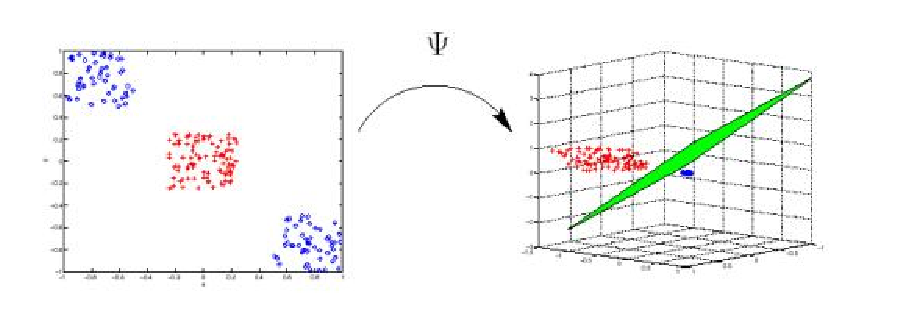
\includegraphics[width=0.6\textwidth]{figures/space_transformation}
	\caption{Non-linear mapping of input examples into high dimensional feature space}
\end{figure}
A drawback of polynomial bases is that the basis functions are "non-local",
meaning that the fitted value of $\hat{y}$ at a given value $x = x_{0}$ depends strongly on 
data values with $x$ far from $x_{0}$.
In modern statistics, polynomial basis-functions are used along with new basis functions,
such as splines, radial basis functions, and wavelets.
These families of basis functions offer a more parsimonious fit for many types of data. 
Adter transformation new observation space is treated as a input for linear regression.

%----------------------------------------------------------------------------------------------------
\subsection{Spline regression}
\FloatBarrier
%----------------------------------------------------------------------------------------------------
\subsection{Radial regression}
\FloatBarrier
%----------------------------------------------------------------------------------------------------
\subsection{Wavelet regression}
\FloatBarrier


%----------------------------------------------------------------------------------------------------
\subsection{Support vector machine}
\FloatBarrier
Support Vector Machines are very specific class of algorithms, 
characterized by usage of kernels, absence of local minima, sparseness of the solution and 
capacity control obtained by acting on the margin, or on number of support vectors, etc.

They were invented by Vladimir Vapnik and his co-workers, 
and first introduced at the Computational Learning Theory (COLT) 1992 conference with the paper.
All these nice features however were already present in machine learning since 1960’s: 
large margin hyper planes usage of kernels, geometrical interpretation of kernels as inner
products in a feature space.
Similar optimization techniques were used in pattern recognition and sparsness techniques 
were widely discussed.
Usage of slack variables to overcome noise in the data and non - separability was also
introduced in 1960s.
However it was not until 1992 that all these features were put together to form the
maximal margin classifier, the basic Support Vector Machine, and not until 1995 that the
soft margin version was introduced.

Support Vector Machine can be applied not only to classification problems but also to the
case of regression.
Still it contains all the main features that characterize maximum margin algorithm:
a non-linear function is leaned by linear learning machine mapping into high dimensional kernel
induced feature space.
The capacity of the system is controlled by parameters that do not depend on the dimensionality
of feature space.

In the same way as with classification approach there is motivation to seek and optimize the
generalization bounds given for regression.
They relied on defining the loss function that ignores errors, which are situated within
the certain distance of the true value.
This type of function is often called – epsilon intensive – loss function. 
The figure below shows an example of one-dimensional linear regression function with – 
epsilon intensive – band. The variables measure the cost of the errors on the training points.
These are zero for all points that are inside the band. 
\begin{figure}[htb] 
	\label{fig:svm1}
	\centering
	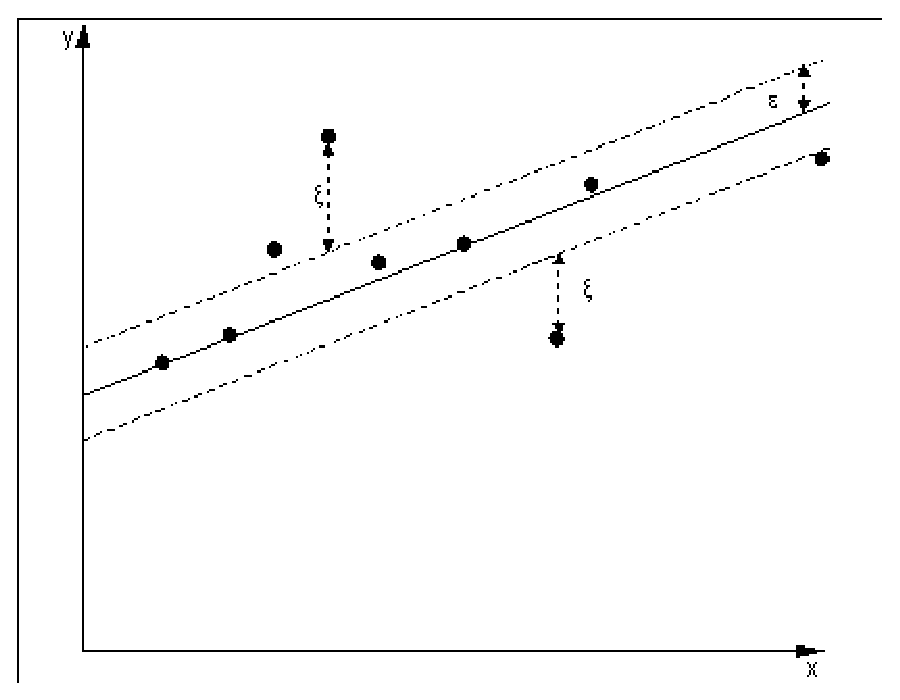
\includegraphics[width=0.6\textwidth]{figures/svm1}
	\caption{One-dimensional linear regression with epsilon intensive band}
\end{figure}

One of the most important ideas in Support Vector Classification and Regression cases is 
that presenting the solution by means of small subset of training points gives enormous 
computational advantages. 
Using the epsilon intensive loss function we ensure existence of the global minimum and at 
the same time optimization of reliable generalization bound.
\begin{figure}[htb] 
	\label{fig:epsilon_band}
	\centering
	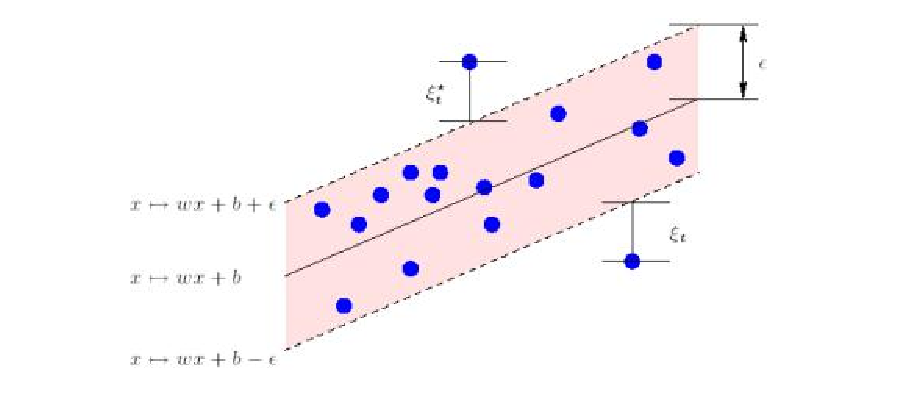
\includegraphics[width=0.6\textwidth]{figures/epsilon_band}
	\caption{Detailed picture of epsilon band with slack variables and selected data points}
\end{figure}
In SVM regression, the inputis first mapped onto a m-dimensional feature space using some 
fixed (nonlinear) mapping, and then a linear model is constructed in this feature space. 
Using mathematical notation, the linear model (in the feature space) is given by:
\begin{equation}
	\label{equ:svm_in}
	h(x) = \sum_{j=1}^{m}\Theta_{j}x_{j} + b
\end{equation}
If the data is assumed to be zero mean bias term $b$ can be dropped which results in following
equation in matrix form:
\begin{equation}
	\label{equ:svm_in_matrix}
	h(x) = \Theta X,
\end{equation}
where $X$ is matrix containing all observations.

The quality of estimation is measured by the loss function.
SVM regression uses a new type of loss function called insensitive loss function proposed 
by Vapnik:
\begin{equation}
	\label{equ:vapnik}
	E(x,y) = \begin{cases}
		0, & |y-h(x)| \leq \varepsilon \\
		|y-h(x)|-\epsilon, & |y-h(x)| > \varepsilon \\
	\end{cases},
\end{equation}
where $\varepsilon$ is \textbf{TODO: CO TO KWA JEST!}.
The empirical risk is:
\begin{equation}
	\label{equ:risk}
	R_{EMP} = \frac{1}{n}\sum_{i=1}^{n}E(x^{(i)}, y^{(i)}),
\end{equation}
where $n$ is observation count.
SVM regression performs linear regression in the high-dimension feature space using 
$\varepsilon$-insensitive loss and, at the same time, tries to reduce model complexity 
by minimizing $\Vert \Theta \Vert^2$. 
This can be described by introducing (non-negative) slack variables 
$\zeta_{i}, \zeta^{\bullet}_{i}$, to measure the deviation of training samples outside
$\varepsilon$-insensitive zone. Thus SVM regression is formulated as minimization 
of the following functional:
\begin{equation}
	\label{equ:svm_functional_pt1}
	\frac{1}{2}\Vert \Theta \Vert^{2} + C\sum_{i=1}^{n}(\zeta_{i}+\zeta^{\bullet}_{i}),
\end{equation}
where \textbf{TODO: WHAT IS THAT (functional)}:
\begin{equation}
	\label{equ:svm_functional_pt2}
	\begin{cases}
		y_{i}-h(x_{i}) \leq \varepsilon + \zeta^{\bullet}_{i}\\
		h(x_{i}) - y_{i} \leq \varepsilon + \zeta_{i}\\
		\zeta_{i},\zeta^{\bullet}_{i} \geq 0
	\end{cases}.
\end{equation}

This optimization problem can transformed into the dual problem and its solution is given by:
\begin{equation}
	\label{equ:svm_dual}
	f(x)=\sum_{i=1}{v}(\alpha_{i}-\alpha^{\bullet}_{i})K(x_{i},x),
\end{equation}
where $v$ is number of support vectors and the $K(x_{i},x)$ is a kernel function such that:
\begin{equation}
	\label{equ:svm_kernel}
	K(x_{i},x) = \sum_{j=1}^{m}g_{j}(x)g_{j}(x_{i}).
\end{equation}

It is well known that SVM generalization performance (estimation accuracy) depends on a 
good setting of meta-parameters parameters $\varepsilon C$,  and the kernel parameters.
The problem of optimal parameter selection is further complicated by the fact that SVM model
complexity (and hence its generalization performance) depends on all three parameters. 
Existing software implementations of SVM regression usually treat SVM meta-parameters 
as user-defined inputs. Selecting a particular kernel type and kernel function parameters 
is usually based on application-domain knowledge and also should reflect distribution of 
input (x) values of the training data.
\begin{figure}[htb] 
	\label{fig:svm_demo1}
	\centering
	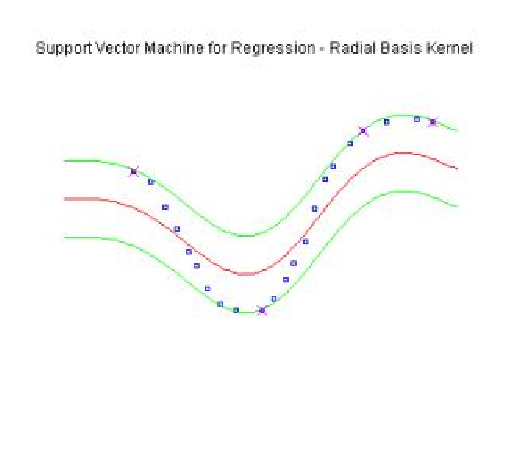
\includegraphics[width=0.6\textwidth]{figures/svm_demo1}
	\caption{Performance of Support Vector Machine in regression case. 
	The epsilon boundaries are given with the green lines. Blue points represent data instances.}
\end{figure}

Parameter $C$ determines the trade off between the model complexity (flatness) and the degree 
to which deviations larger than $\varepsilon$  are tolerated in optimization formulation.
For example, if $C$ is too large (infinity), then the objective is to minimize the empirical 
risk only, without regard to model complexity part in the optimization formulation.
Parameter controls the width of the $\varepsilon$-insensitive zone, used to fit the training data.
The value of $\varepsilon$ can affect the number of support vectors used to construct the
regression function. 
The bigger $\varepsilon$ , the fewer support vectors are selected. On the other hand, 
bigger $\varepsilon$-values results in more ‘flat’ estimates.
Hence, both $C$ and $\varepsilon$-values affect model complexity (but in a different way).
\begin{figure}[htb] 
	\label{fig:svm_demo2}
	\centering
	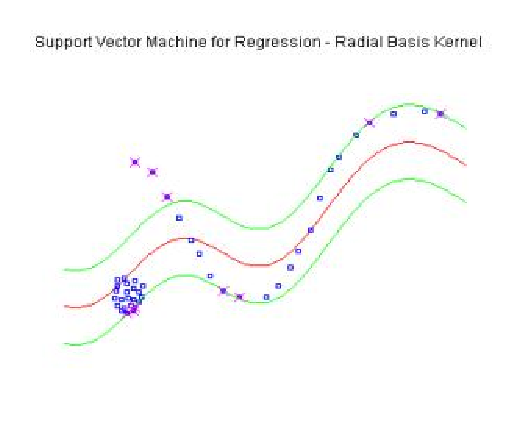
\includegraphics[width=0.6\textwidth]{figures/svm_demo2}
	\caption{Performance of Support Vector Machine in regression case.
	The epsilon boundaries are given with the green lines. Blue points represent data instances.}
\end{figure}

Additional instances are introduced in this case and after being supplied to the model are 
inside epsilon band. The regression function has changed. 
However this makes some points that were initially inside the interval to be misclassified.
\begin{figure}[htb] 
	\label{fig:svm_demo3}
	\centering
	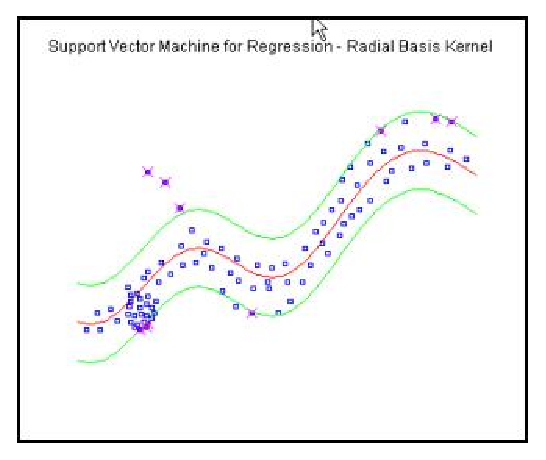
\includegraphics[width=0.6\textwidth]{figures/svm_demo3}
	\caption{Performance of Support Vector Machine in regression case.
	The epsilon boundaries are given with the green lines. Blue points represent data instances}
\end{figure}
Introducing new data instances that are located inside the epsilon band,
do not influence the structure of the model.
It can be seen that regression function has not changed at all.
One of the advantages of Support Vector Machine, and Support Vector Regression as the part of it,
is that it can be used to avoid difficulties of using linear functions in the high dimensional 
feature space and optimization problem is transformed into dual convex quadratic programmes.
In regression case the loss function is used to penalize errors that are grater than threshold 
- $\varepsilon$.
Such loss functions usually lead to the sparse representation of the decision rule,
giving significant algorithmic and representational advantages. 

%====================================================================================================
\section{Gradient based optimization}
\FloatBarrier
\label{sec:gradient}
How can you minimize a function $\ell$ if you don't know much about it? 
The trick is to assume it is much simpler than it really is. This can be done with 
Taylor's approximation. Provided that the norm $\Vert s \Vert^{2}$ is small 
(i.e. $w + s$ is very close to $w$), we can approximate the function $\ell (w+s)$ by its 
first: 
\begin{equation}
	\label{equ:first_and_second_derivative}
	\ell(w+s) \approx \ell(w) + g(w)^{\top}s,
\end{equation}
end second derivative:
\begin{equation}
	\label{equ:first_and_second_derivative}
	\ell(w+s) \approx \ell(w) + g(w)^{\top}s + \frac{1}{2}s^{\top}H(w)s,
\end{equation}
where $g(w)=\nabla \ell (w)$ is the gradient and $H(w)=\nabla 2 \ell (w)$ 
is the Hessian of $\ell$.
Both approximations are valid if $\Vert s\Vert^{2}$ is small, but the second one assumes that
$\ell$ is twice differentiable and is more expensive to compute but also more accurate 
than only using gradient. 

%----------------------------------------------------------------------------------------------------
\subsection{Gradient descent}
\FloatBarrier
In gradient descent we only use the gradient (first order). 
In other words, we assume that the function $\ell$ around $w$ is linear and behaves like 
$\ell(w)+g(w)^{\top}s$. Our goal is to find a vector $s$ that minimizes this function. 
In steepest descent we simply set
\begin{equation}
	\label{equ:delta_weights}
	s=-\alpha g(w),
\end{equation}
where $\alpha$ is learning rate.
Setting the learning rate $\alpha$ is a dark art. Only if it is sufficiently small will gradien
t descent converge (see the first figure below).
If it is too large the algorithm can easily diverge out of control (see the second figure below).
A safe (but sometimes slow) choice is to set $\alpha = \frac{t_{0}}{t}$, which guarantees that it
will eventually become small enough to converge (for any initial value $t_{0}>0$). 
\begin{figure}[htb] 
	\label{fig:gradient_converge}
	\centering
	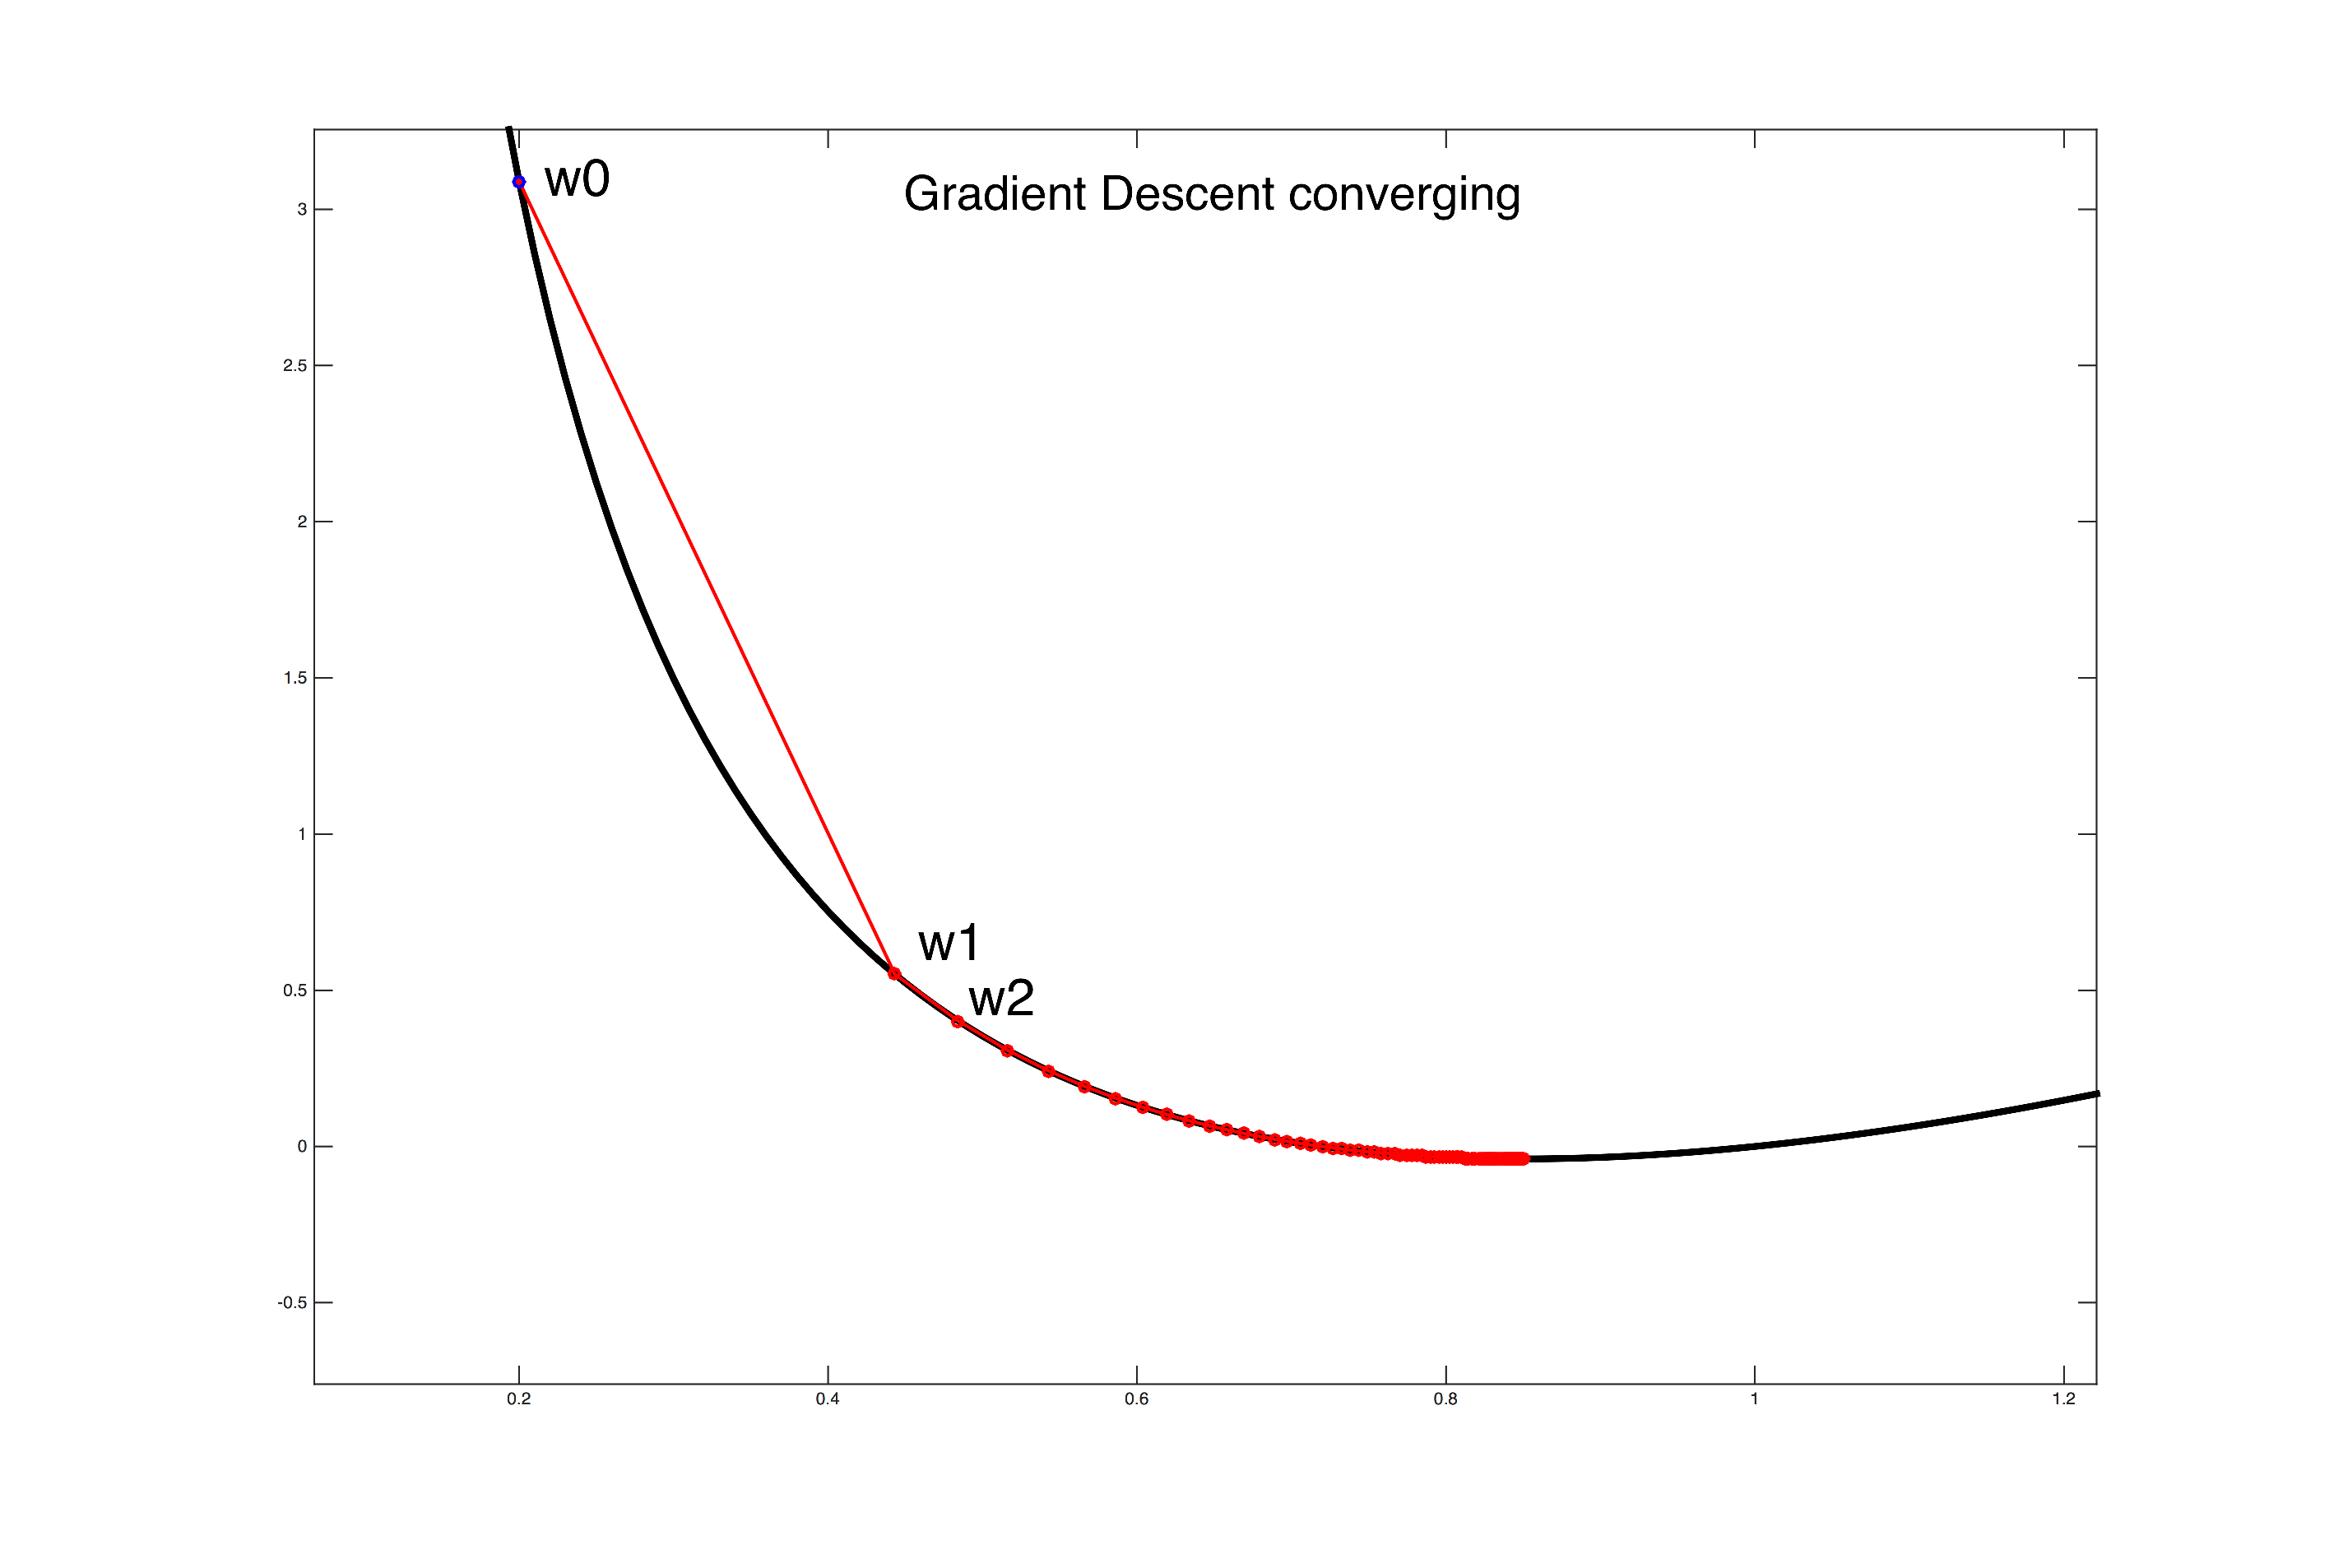
\includegraphics[width=0.6\textwidth]{figures/gradient_converge}
	\caption{Gradient descent converging on minimum}
\end{figure}
\begin{figure}[htb] 
	\label{fig:gradient_skip}
	\centering
	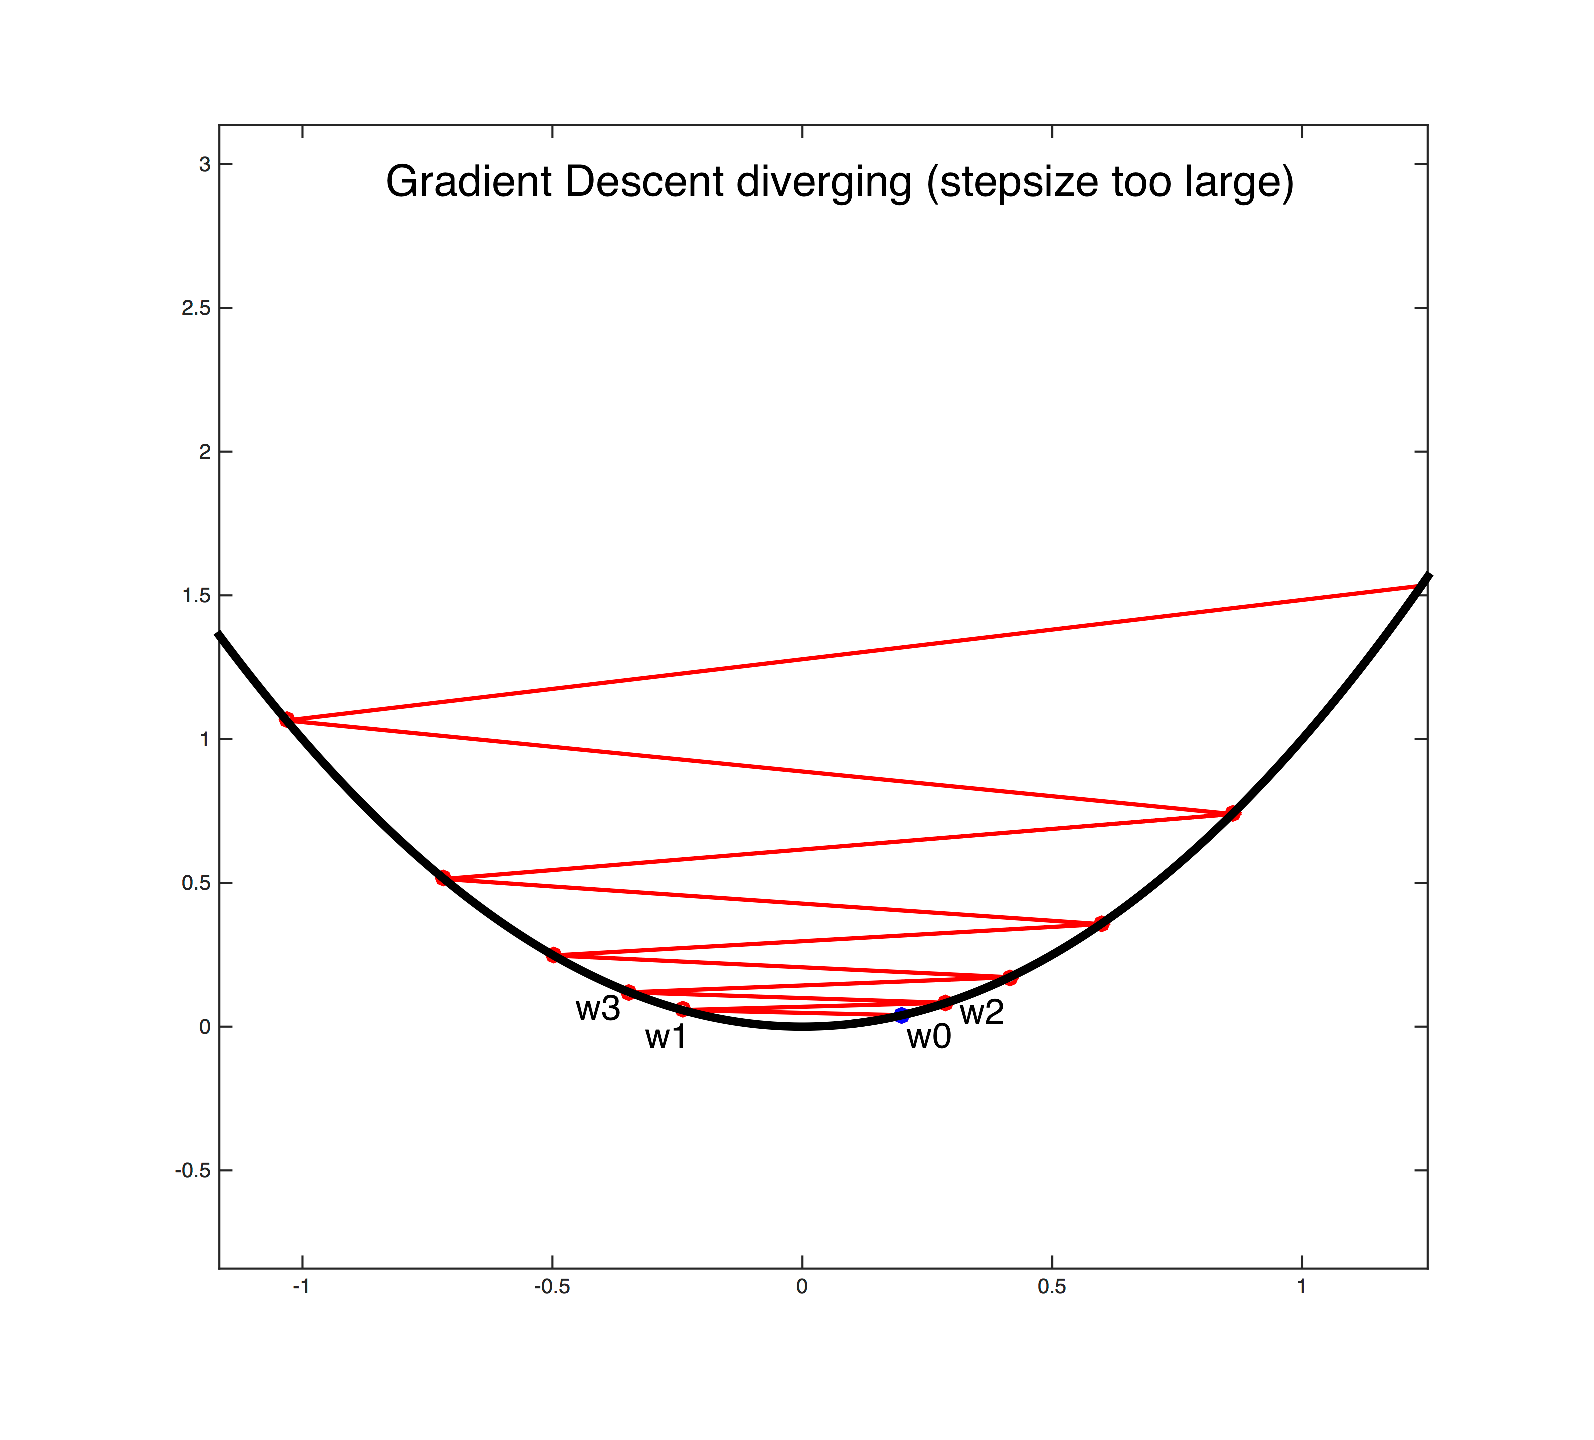
\includegraphics[width=0.6\textwidth]{figures/gradient_skip}
	\caption{Gradient descent converging on minimum}
\end{figure}


%----------------------------------------------------------------------------------------------------
\subsection{Momentum based gradient descent}
\FloatBarrier
The problem with gradient descent is that the weight update at a moment is governed by the
learning rate and gradient at that moment only. 
It doesn’t take into account the past steps taken while traversing the cost space.
It leads to the following problems.
\begin{enumerate}
	\item The gradient of the cost function at saddle points( plateau) is negligible or zero,
		which in turn leads to small or no weight updates. 
		Hence, the network becomes stagnant, and learning stops
    \item The path followed by Gradient Descent is very jittery even when 
		operating with mini-batch mode
\end{enumerate}
Consider the below cost surface.
\begin{figure}[htb] 
	\label{fig:gradient_problem}
	\centering
	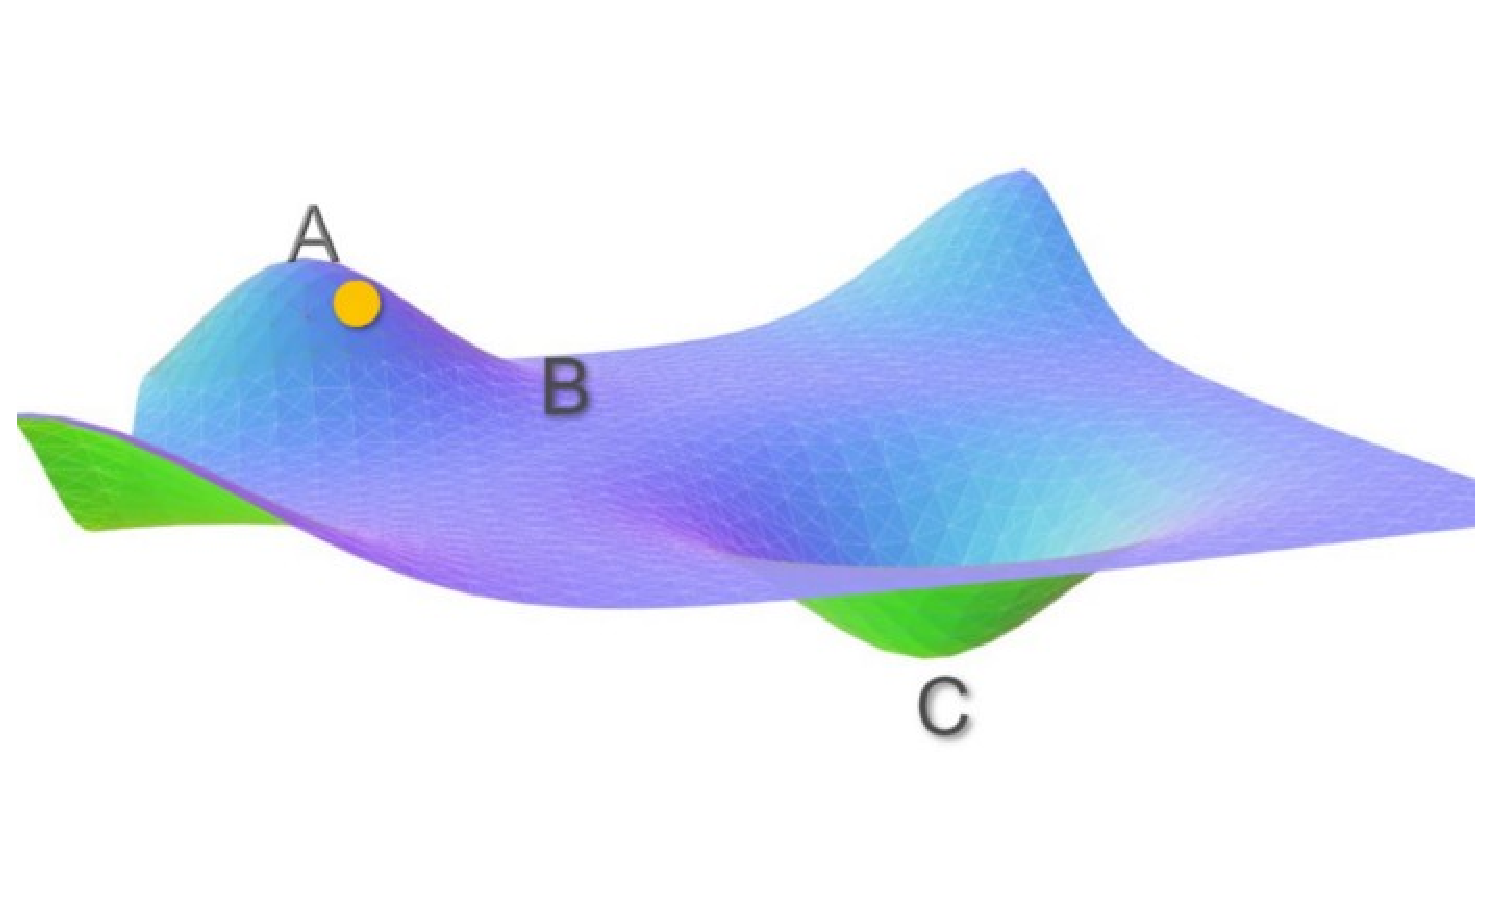
\includegraphics[width=0.6\textwidth]{figures/gradient_problem}
	\caption{Gradient will have problems}
\end{figure}
Let’s assume the initial weights of the network under consideration correspond to point A. 
With gradient descent, the Loss function decreases rapidly along the slope AB as the gradient
along this slope is high.
But as soon as it reaches point B the gradient becomes very low. The weight updates around B 
is very small. Even after many iterations, the cost moves very slowly before getting stuck at a
point where the gradient eventually becomes zero.
In this case, ideally, cost should have moved to the global minima point C,
but because the gradient disappears at point B, we are stuck with a sub-optimal solution.
Now, Imagine you have a ball rolling from point A. The ball starts rolling down slowly and gathers
some momentum across the slope AB. 
When the ball reaches point B, it has accumulated enough momentum to push itself across the
plateau region B and finally following slope BC to land at the global minima C.
To account for the momentum, we can use a moving average over the past gradients.
In regions where the gradient is high like AB, weight updates will be large. Thus, in a way we
are gathering momentum by taking a moving average over these gradients.
But there is a problem with this method, it considers all the gradients over iterations with 
equal weightage. The gradient at $t=0$ has equal weightage as that of the gradient at
current iteration $t$. We need to use some sort of weighted average of the past gradients such
that the recent gradients are given more weightage.
This can be done by using an Exponential Moving Average(EMA).
An exponential moving average is a moving average that assigns a greater weight on the most 
recent values. The EMA for a series Y may be calculated recursively:
\begin{equation}
	\label{equ:ema}
	S(t) = /beta S(t-1)+(1-\beta)Y(t),
\end{equation}
where the coefficient $\beta \in <0,1>$ represents the degree of weighting increase,  Y(t) is
the value at a period t and  S(t) is the value of the EMA at any period t.
First algorithm step is assumed at $t=1$ and $S(0)=0$.
In our case of a sequence of gradients, the new weight update equation at iteration $t$ becomes:
\begin{equation}
	\label{equ:momentum_update}
	v(t) = \beta v(t-1)+(1-\beta)\delta(t),
\end{equation}
where $v(t)$ is the new weight update done at iteration $t$ $\beta$ is momentum constant and
$\delta(t)$: is the gradient at iteration $t$.
With assumption that $v(0)=0$ change of waights at step $n$ can be described as:
\begin{equation}
	\label{equ:momentum_update_sum}
	v(n) = (1-\beta)\sum_{t=1}^{n}\beta^{n-1}\delta(t).
\end{equation}
In the cost surface shown earlier let's zoom into point C.
With gradient descent, if the learning rate is too small, the weights will be updated very 
slowly hence convergence takes a lot of time even when the gradient is high. 
This is shown in the left side image below. If the learning rate is too high cost
oscillates around the minima as shown in the right side image below.

Let's look at the last summation equation of the momentum again.
When all the past gradients have the same sign the summation term will become large and we 
will take large steps while updating the weights.
Along the curve BC, even if the learning rate is low, all the gradients along the curve will 
have the same direction(sign) thus increasing the momentum and accelerating the descent.
When some of the gradients have $+ve$ sign whereas others have $-ve$ the summation term will
become small and weight updates will be small. 
If the learning rate is high, the gradient at each iteration around the valley C will
alter its sign between $+ve$ and $-ve$ and after few oscillations, the sum of past gradients 
will become small. Thus, making small updates in the weights from there on and damping the 
oscillations.

This to some amount addresses our second problem. Gradient Descent with Momentum takes small 
steps in directions where the gradients oscillate and take large steps along the direction where
the past gradients have the same direction(same sign).

%----------------------------------------------------------------------------------------------------
\subsection{Stochastic gradient descent}
\FloatBarrier
Stochastic gradient descent (often abbreviated SGD) is an iterative method for optimizing an
objective function with suitable smoothness properties (e.g. differentiable or subdifferentiable).
It can be regarded as a stochastic approximation of gradient descent optimization, since it 
replaces the actual gradient (calculated from the entire data set) by an estimate thereof 
(calculated from a randomly selected subset of the data). Especially in high-dimensional 
optimization problems this reduces the computational burden,
achieving faster iterations in trade for a lower convergence rate.
While the basic idea behind stochastic approximation can be traced back to the Robbins–Monro 
algorithm of the 1950s, stochastic gradient descent has become an important optimization
method in machine learning. 
In stochastic (or "on-line") gradient descent, the true gradient  is approximated by a gradient
at a single example.
As the algorithm sweeps through the training set, it performs the above update for each training
example. Several passes can be made over the training set until the algorithm converges.
If this is done, the data can be shuffled for each pass to prevent cycles.
Typical implementations may use an adaptive learning rate so that the algorithm converges

%----------------------------------------------------------------------------------------------------
\subsection{Adaptive gradient algorithm (AdaGrad)}
\FloatBarrier
AdaGrad is simply just an optimization method based off of the Proximal Point Algorithm 
(otherwise known as the Gradient Descent algorithm), specifically the Stochastic version
of gradient descent.
The intention behind the formulation of AdaGrad is because SGD (stochastic gradient descent) 
converges slowly in the cases when features of our model are significantly more 
important than others. 
This is because the original SGD algorithm treats all factors equally, regardless of how much
each factor contributes towards the actual models outputs.

Seen below, we can recognize that the stochastic gradient descent algorithm takes a large
amount of time in order to find the optimal solution because of the constant jumping back and
forth on the expected gradient (seen Left). 
On the otherhand, if we were to average all of the iterates in SGD (not AdaGrad), 
we can find a much quicker optimization and decrease the amount of backtracking done.

Now consider a case where we have an extremely wide problem domain, most likely due to a
feature having an exaggerated effect on the domain.
Seen below, we can see that the standard proximal gradient method (SGD) ends up jumping back and 
forth because it is a poorly conditioned problem.
On the other hand, we can see the AdaGrad variant (which somewhat fixes the poor conditioning of 
the problem) will end up getting to the optimal in a significantly smaller number of steps.
The original SGD algorithm’s update method defines the update rule as:
\begin{equation}
	\label{equ:SGD_equ}
	x^{(k+1)} = argmin_{x\in \chi}\{\langle g^{(k)},x\rangle + frac{1}{2\alpha_{k}}
	\Vert x-x^{(k)}\Vert_{2}^{2}\}.
\end{equation}
This version of the algorithm has a general convergence rate of $O(\frac{1}{T})$.
AdaGrad takes advantage of the matrix norm, in our case, $B$ will be a positive
definite matrix such that:
\begin{equation}
	\label{equ:definite_matrix}
	\Vert  x \Vert_{B}^{2} = x^{T}Bx \geq 0.
\end{equation}
This matrix $B$ has a list of diagonal terms that will modify the update rule of SGD such that:
\begin{equation}
	\label{equ:modified_SGD}
	x^{(k+1)} = argmin_{x\in \chi}\{\langle \nabla f(x^{(k)} ,x\rangle + frac{1}{2\alpha_{k}}
	\Vert x-x^{(k)}\Vert_{B}^{2}\},
\end{equation}
which is equivalent to an update rule of:
\begin{equation}
	\label{equ:mod_sgd_equ}
	x^{(k+1)} = x^{(k)} - \alpha B^{-1} \nabla f(x^{(k)}).
\end{equation}

As can be seen when compared to the original update rule, we have introduced the diagonal matrix
$B$ in order to converge more quickly because of the reliance on features that are
more exaggerated than less important features.
Now the question is how we can best approximate $B$, since it is unknown to the user.
AdaGrad now extends the SGD algorithm by defining within iteration $k$:
\begin{equation}
	\label{equ:adagrad_extension}
	G^{(k)} = diag[\sum_{i=1}^{k}g^{(i)}(g^{(i)})^{T}]^{1/2},
\end{equation}
We can define $G^{(k)}$ as a diagonal matrix with entries:
\begin{equation}
	\label{equ:adagrad_matrix}
	G^{(k)}_{jj} = \sqrt{\sum_{i=1}^{k} (g_j^{(i)})^2}
\end{equation}
Therefore modifying our previous modified update rule to be our final update rule for Adagrad:
\begin{equation}
	\label{equ:adagrad_opt}
	x^{(k+1)} = \text{argmin}_{x \in \chi} \{ \langle \nabla f(x^{(k)}), x \rangle + 
	\frac{1}{2 \alpha_k} \lvert \lvert x - x^{(k)} \rvert \rvert_{G^{(k)}}^2 \}
\end{equation}
which is equivalent to an update rule of:
\begin{equation}
	\label{equ:adagrad_opt_equiv}
	x^{(k+1)} = x^{(k)} - \alpha G^{-1} \nabla f(x^{(k)})
\end{equation}

%----------------------------------------------------------------------------------------------------
\subsection{RMProp and RMSProp}
\FloatBarrier
RMSprop— is unpublished optimization algorithm designed for neural networks, first proposed by
Geoff Hinton in lecture 6 of the online course “Neural Networks for Machine Learning”.
RMSprop lies in the realm of adaptive learning rate methods, which have been growing in
popularity in recent years, but also getting some criticism. 
It’s famous for not being published, yet being very well-known; most deep learning framework 
include the implementation of it out of the box.

There are two ways to introduce RMSprop. First, is to look at it as the adaptation of rprop
algorithm for mini-batch learning. 
It was the initial motivation for developing this algorithm. Another way is to look at its 
similarities with Adagrad and view RMSprop as a way to deal with its radically diminishing
learning rates.
I’ll try to hit both points so that it’s clearer why the algorithm works.

Let’s start with understanding rprop — algorithm that’s used for full-batch optimization. 
Rprop tries to resolve the problem that gradients may vary widely in magnitudes.
Some gradients may be tiny and others may be huge, which result in very difficult problem —
trying to find a single global learning rate for the algorithm. 
If we use full-batch learning we can cope with this problem by only using the sign 
of the gradient.
With that, we can guarantee that all weight updates are of the same size. 
This adjustment helps a great deal with saddle points and plateaus as we take big enough steps
even with tiny gradients. 
Note, that we can’t do that just by increasing the learning rates, because steps we take with 
large gradients are going to be even bigger, which will result in divergence.
Rprop combines the idea of using the sign of the gradient with the idea of adapting step size
individualy for each weight.
So, instead of looking at the magnitude of the gradient, we’ll look at the step size that’s 
defined for that particular weight.
And that step size adapts individually over time, so that we accelerate learning in the
direction that we need. To adjust the step size for some weight, the following algorithm is used
\begin{enumerate}
    \item First, we look at the signs of the last two gradients for the weight.
    \item If they have the same sign, that means, we’re going in the right direction,
		and should accelerate it by a small fraction, meaning we should increase the step size
		multiplicatively(e.g by a factor of 1.2). 
		If they’re different, that means we did too large of a step and jumped over a
		local minima, thus we should decrease the step size multiplicatively(e.g. by a
		factor of 0.5).
    \item Then, we limit the step size between some two values. These values really depend on
		your application and dataset, good values that can be for default are 50 and a millionth, 
		which is a good start.
    \item Now we can apply the weight update.
\end{enumerate}

Rprop doesn’t really work when we have very large datasets and need to perform mini-batch weights
updates. 
Why it doesn’t work with mini-batches ? Well, people have tried it, but found it hard to make 
it work.
The reason it doesn’t work is that it violates the central idea behind stochastic gradient
descent, which is when we have small enough learning rate,
it averages the gradients over successive mini-batches.
Consider the weight, that gets the gradient 0.1 on nine mini-batches, and the gradient of -0.9 on
tenths mini-batch.
What we’d like is to those gradients to roughly cancel each other out, so that the stay
approximately the same.
But it’s not what happens with rprop. With rprop, we increment the weight 9 times and decrement
only once, so the weight grows much larger.

To combine the robustness of rprop (by just using sign of the gradient), efficiency we get 
from mini-batches, and averaging over mini-batches which allows to combine gradients in the
right way, we must look at rprop from different perspective.
Rprop is equivalent of using the gradient but also dividing by the size of the gradient,
so we get the same magnitude no matter how big a small that particular gradient is.
The problem with mini-batches is that we divide by different gradient every time, so why not force
the number we divide by to be similar for adjacent mini-batches ?
The central idea of RMSprop is keep the moving average of the squared gradients for each weight.
And then we divide the gradient by square root the mean square. 
Which is why it’s called RMSprop(root mean square). With math equations the update rule
looks like this:
\begin{equation}
	\label{equ:rmsprop1}
	E[g^{2}]_{t} = \beta E[g^{2}]_{t-1}+(1-\beta)(\frac{\delta C}{\delta w})^{2},
\end{equation}
\begin{equation}
	\label{equ:rmsprop2}
	w_{t} = w_{t-1} - \frac{\eta}{\sqrt{E[g^{2}]_{t}}} \frac{\delta C}{\delta w},
\end{equation}
where $E[g]$ is moving average of squared gradients. $\frac{\delta C}{\delta w}$ is gradient of
the cost function with respect to the weight, $\eta$  learning rate and $\beta$  moving average
parameter.
As you can see from the above equation we adapt learning rate by dividing by the root of
squared gradient, but since we only have the estimate of the gradient on the current mini-batch,
wee need instead to use the moving average of it.
%----------------------------------------------------------------------------------------------------
\subsection{Adaptive Moment Estimation (Adam)}
\FloatBarrier
Adam, derived from Adaptive Moment Estimation, is an optimization algorithm.
The Adam optimizer makes use of a combination of ideas from other optimizers.
Similar to the momentum optimizer, Adam makes use of an exponentially decaying average of 
past gradients.
Thus, the direction of parameter updates is calculated in a manner similar to that of
the momentum optimizer.
Adam also employs an exponentially decaying average of past squared gradients in order to
provide an adaptive learning rate. 
Thus, the scale of the learning rate for each dimension is calculated in a manner similar to 
that of the RMSProp optimizer.
The similarity of the Adam optimizer to the momentum and RMSProp optimizers is
immediately clear upon examining the equations defining the Adam optimizer.
\begin{equation}
	m = \beta_{1}m - (1-\beta_{1})\nabla_{\Theta}J(\Theta),
\end{equation}
\begin{equation}
	s = \beta_{2}s+(1-\beta_{2})\nabla_{\Theta}J(\Theta)\odot \nabla_{\Theta}J(\Theta),
\end{equation}
\begin{equation}
	\hat{m} = \frac{m}{1-\beta^{t}_{1}},
\end{equation}
\begin{equation}
	\hat{s} = \frac{s}{1-\beta^{t}_{2}},
\end{equation}
\begin{equation}
	\Theta = \Theta + \eta \hat{m} \oslash \sqrt{\hat{s}+c},
\end{equation}
where $\odot$ denotes the Hadamard product (element-wise multiplication) and $\oslash$ denotes
Hadamard division (element-wise division).

$\epsilon$ is the smoothing term used to prevent division by zero.

The vector $\hat{m}$ is used to provide the update direction for each parameter.
As this vector is not equal to $\nabla \Theta J(\Theta)$ but an average over the past gradients,
the update direction has ‘momentum’. In practice the inclusion of momentum often speeds up 
convergence, but may cause oscillations around the minimum. 
\begin{figure}[htb] 
	\label{fig:adam_starting_momentum}
	\centering
	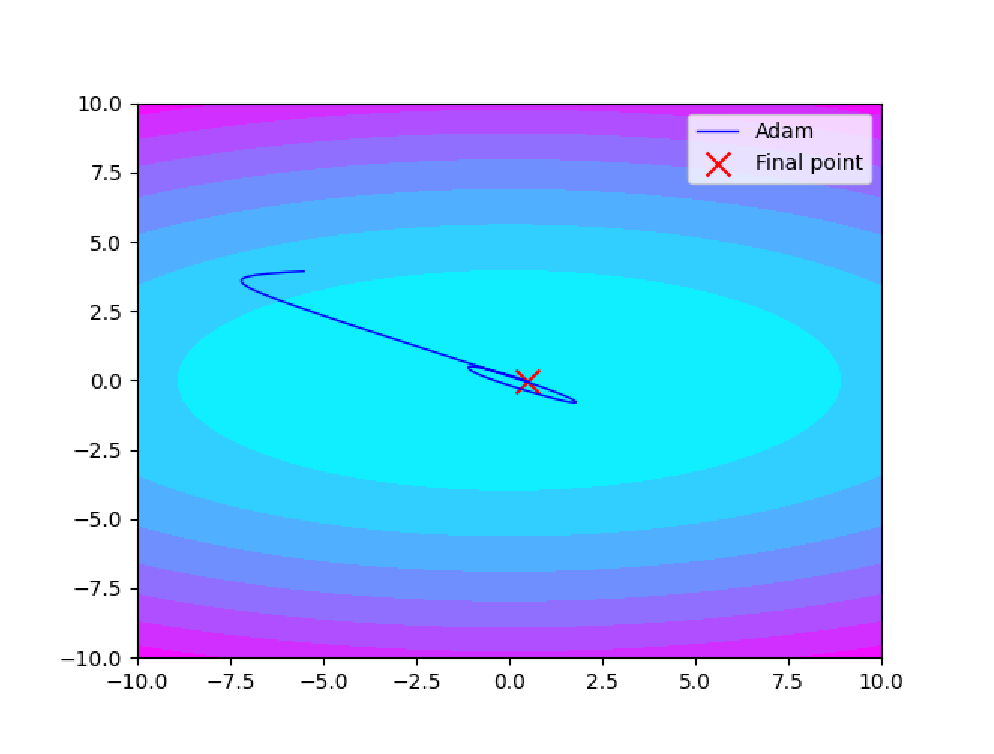
\includegraphics[width=0.6\textwidth]{figures/adam_starting_momentum}
	\caption{The path followed by the Adam optimizer with a large initial momentum vector}
\end{figure}
The path followed by the Adam optimizer with a large initial momentum vector.
An example of the effect momentum has on an optimizer is illustrated in figure 1. 
In this example I set a large (negative) initial value for the first parameter in 
the momentum vector.
This forced the optimizer to initially move left in figure 1, even though this direction 
increases loss. 
This shows that given a large enough momentum vector, the momentum will be able to push the loss
out of local optima and into more optimal solutions if they are present.
The vector $s$ is used to provide an adaptive learning rate. 
This vector stores an exponentially decaying average of the past squared gradients.
Thus, the values of $s$ will be much larger for dimensions with large gradients. 
As a result of this, when the updates are scaled by $\frac{1}{\sqrt{\hat{s}+\epsilon}}$ it will
cause the learning rate to be much smaller for dimensions with large gradients.
This is how $\hat{s}$ is used to provide an adaptive learning rate. 
The use of an adaptive learning rate helps to direct updates towards the optimum.
\begin{figure}[htb] 
	\label{fig:adam}
	\centering
	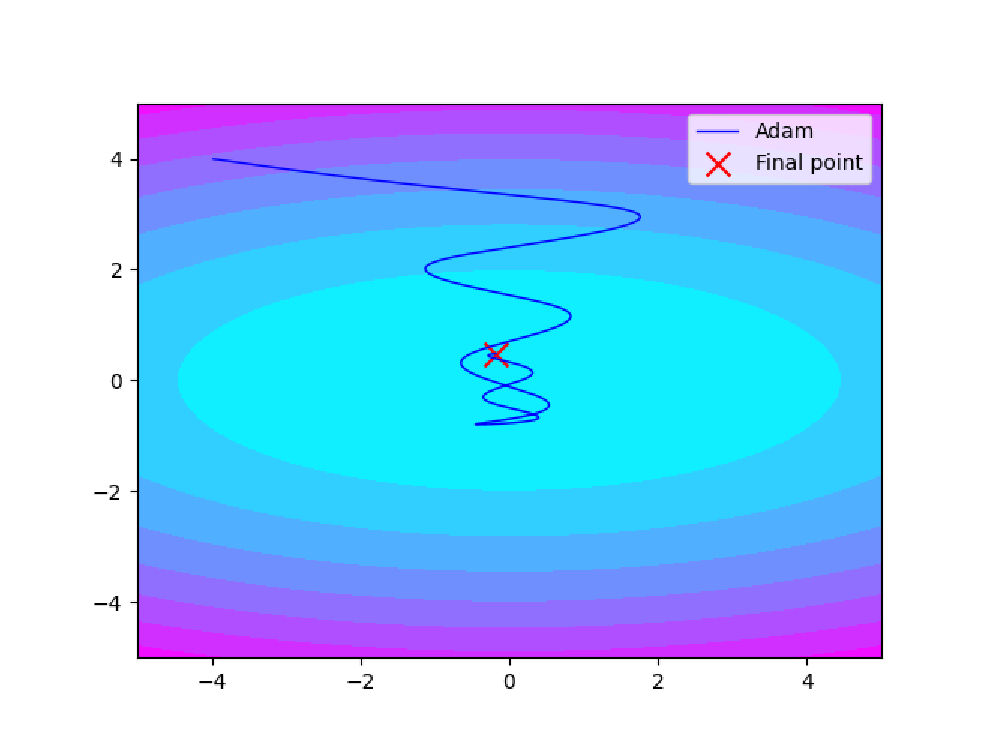
\includegraphics[width=0.6\textwidth]{figures/adam}
	\caption{The path followed by the Adam optimizer with a large initial momentum vector}
\end{figure}


%----------------------------------------------------------------------------------------------------
\subsection{Newton's Method}
\FloatBarrier
Newton's method assumes that the loss $\ell$ is twice differentiable and uses the approximation 
with Hessian (2nd order Taylor approximation).
The Hessian Matrix contains all second order partial derivatives and is defined as:
\begin{equation}
	\label{equ:hessian}
	H(w) = \left( \begin{array}{c c c c}
		\frac{\partial^{2}\ell}{\partial w_{1}^{2}}&
		\frac{\partial^{2}\ell}{\partial w_{1}w_{2}}& \cdots&
		\frac{\partial^{2}\ell}{\partial w_{1}w_{n}}\\

		\frac{\partial^{2}\ell}{\partial w_{2}w_{1}}&
		\frac{\partial^{2}\ell}{\partial w_{2}^{2}}& \cdots&
		\frac{\partial^{2}\ell}{\partial w_{2}w_{n}}\\

		\vdots& \vdots& \ddots& \hdots\\

		\frac{\partial^{2}\ell}{\partial w_{n}w_{1}}&
		\frac{\partial^{2}\ell}{\partial w_{n}w_{2}}& \cdots&
		\frac{\partial^{2}\ell}{\partial w_{n}^{2}}\\
	\end{array} \right),
\end{equation}
because the convexity of $\ell$, it is always a symmetric square matrix and positive
semi-definite. 
A symmetric matrix $M$ is positive semi-definite if it has only non-negative eigenvalues or, 
equivalently, for any vector $x$ we must have $x^{T}Mx\geq 0$.

It follows that the approximation
\begin{equation}
	\label{equ:newton_approx}
	\ell(w+s) \approx \ell(w) + g(w)^{T}s + 0.5s^{T}H(w)s,
\end{equation}
describes a convex parabola, and we can find its minimum by solving the following 
optimization problem: 
\begin{equation}
	\label{equ:newton_opt}
	argmin[\ell(w) + g(w)^{T}s + 0.5s^{T}H(w)s].
\end{equation}
To find the minimum of the objective, we take its first derivative with respect to $s$,
equate it with zero, and solve for $s$:
\begin{equation}
	\label{equ:newton_opt_solved}
	g(w) + H(w)s = 0 \to s = -H^{-1}(w)g(w).
\end{equation}
This choice of s converges extremely fast if the approximation is sufficiently accurate and the 
resulting step sufficiently small.
Otherwise it can diverge. Divergence often happens if the function is flat or almost flat with 
respect to some dimension. In that case the second derivatives are close to zero, and their
inverse becomes very large - resulting in gigantic steps.
Different from gradient descent, here there is no step-size that guarantees that steps are 
all small and local. 
As the Taylor approximation is only accurate locally, large steps can move the current estimates
far from regions where the Taylor approximation is accurate. 
\begin{figure}[htb] 
	\label{fig:gradient_newton}
	\centering
	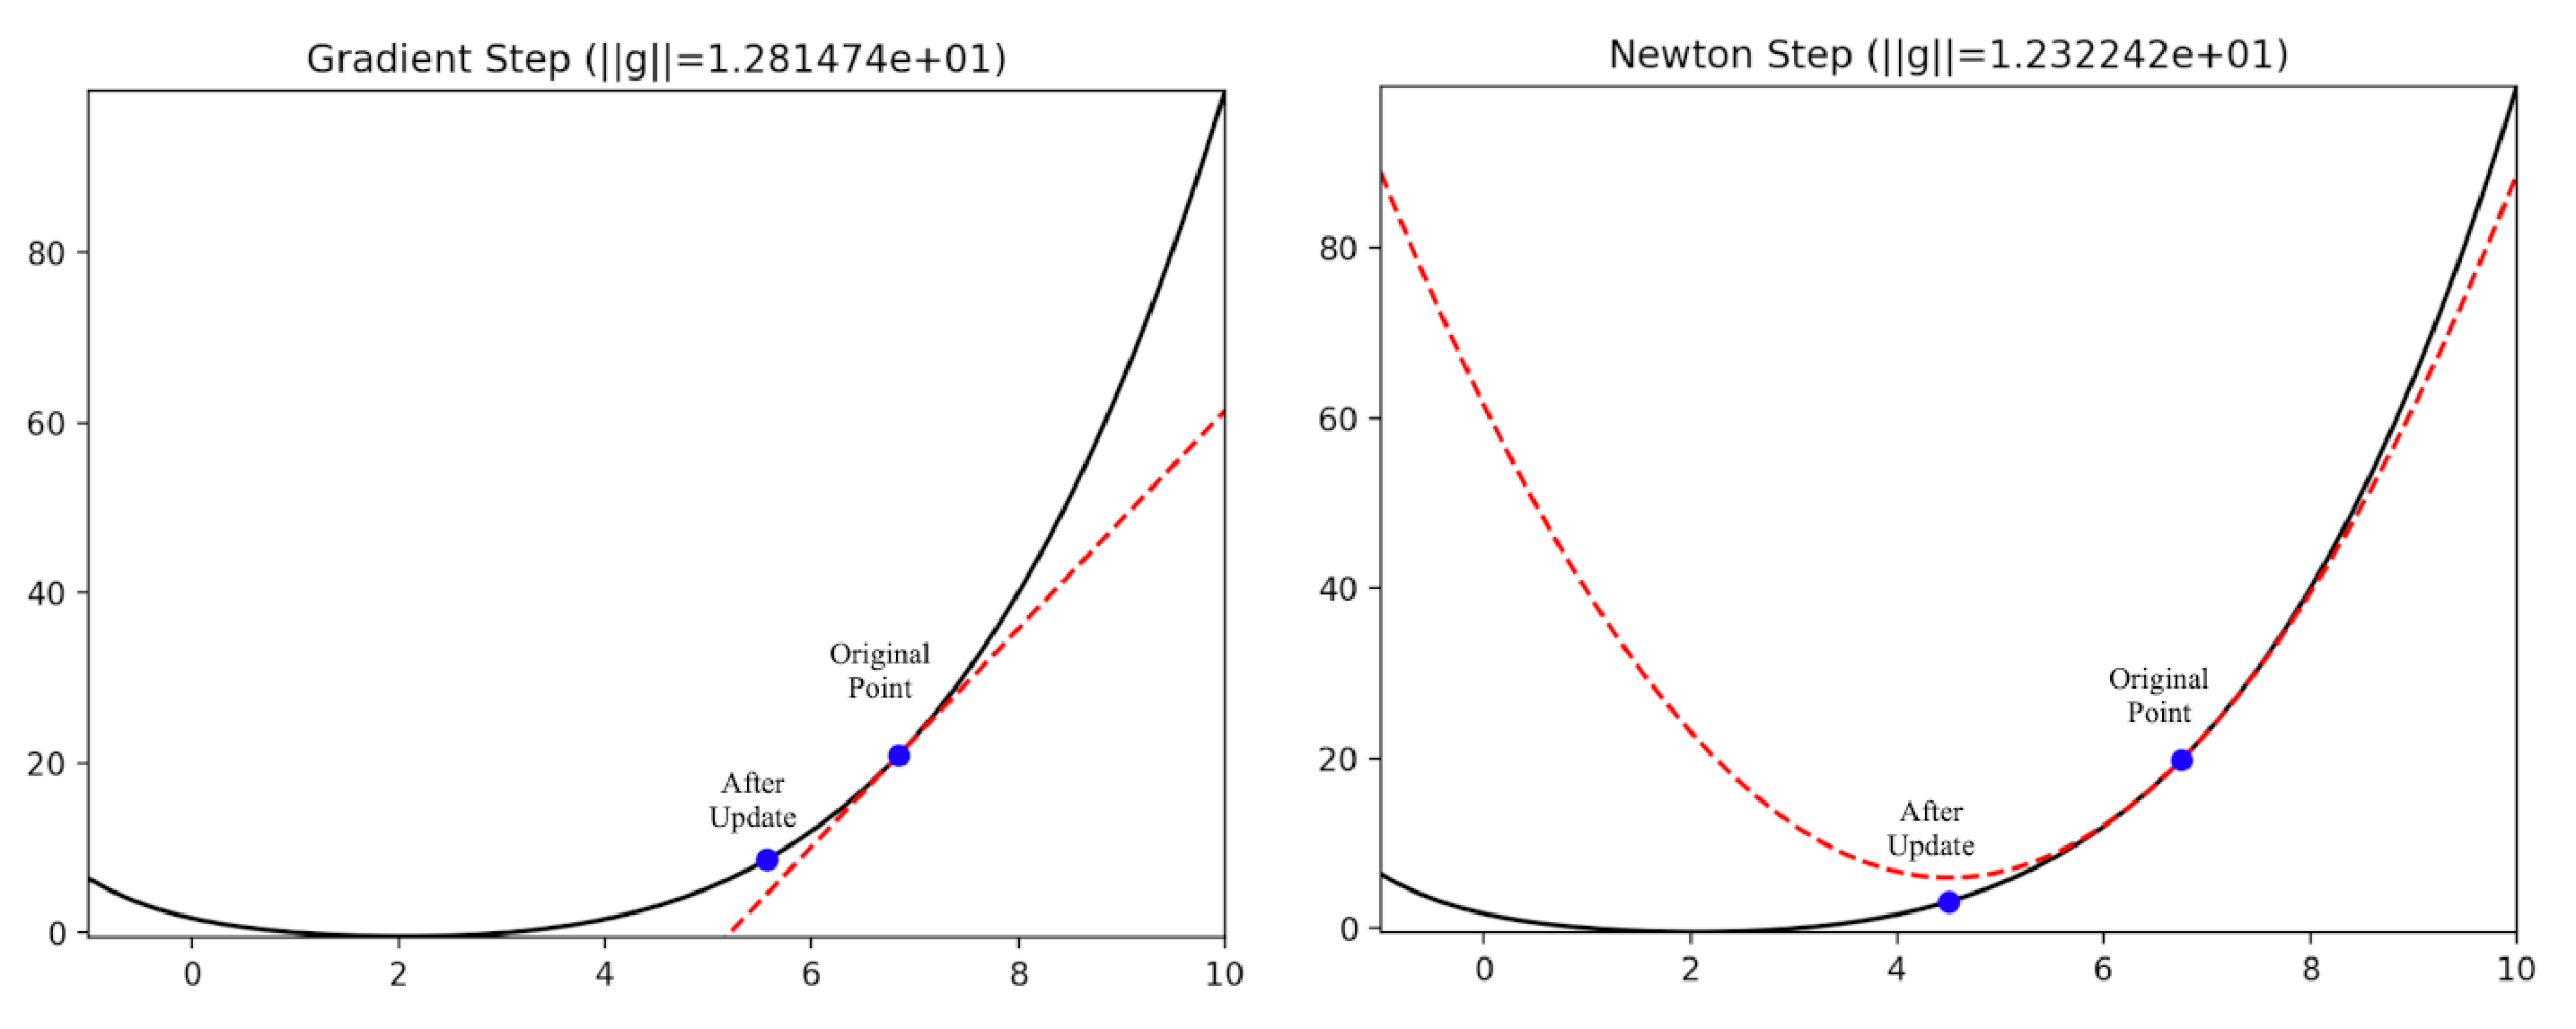
\includegraphics[width=\textwidth]{figures/gradient_newton}
	\caption{A gradient descent step (left) and a Newton step (right) on the same function}
\end{figure}
To avoid divergence of Newton's method, a good approach is to start with gradient descent 
(or even stochastic gradient descent) and then finish the optimization Newton's method.
Typically, the second order approximation, used by Newton's Method, is more likely to be
appropriate near the optimum.

%====================================================================================================
\section{Neural networks}

%----------------------------------------------------------------------------------------------------
\subsection{Neural networks as biological information processing systems}
\FloatBarrier
The basic conducting element in the nervous system is the nerve cell, or neuron.
A neuron has a cell body, dendrite, and axon. The cell body contains many of the organelles 
vital to maintain the cells structure and function, including the nucleus and and is considered the
tropic center of the nerve cell.
The dendrites extend from the cell body and increase the receptive surface of the neuron.
The axon leaves the cell body and connects to other cells. Axons are covered by a lipoproteinaceous
membrane called myelin that insulates the axons from the fluids in the central nervous system.
The site of contact between the axon of one nerve cell and the dendrites and cell body of another 
neuron is the synapse. The cells in the nervous system are classified based on their shapes:
unipolar, bipolar, and multipolar. 
\begin{figure}[htb] 
	\label{fig:neurons}
	\centering
	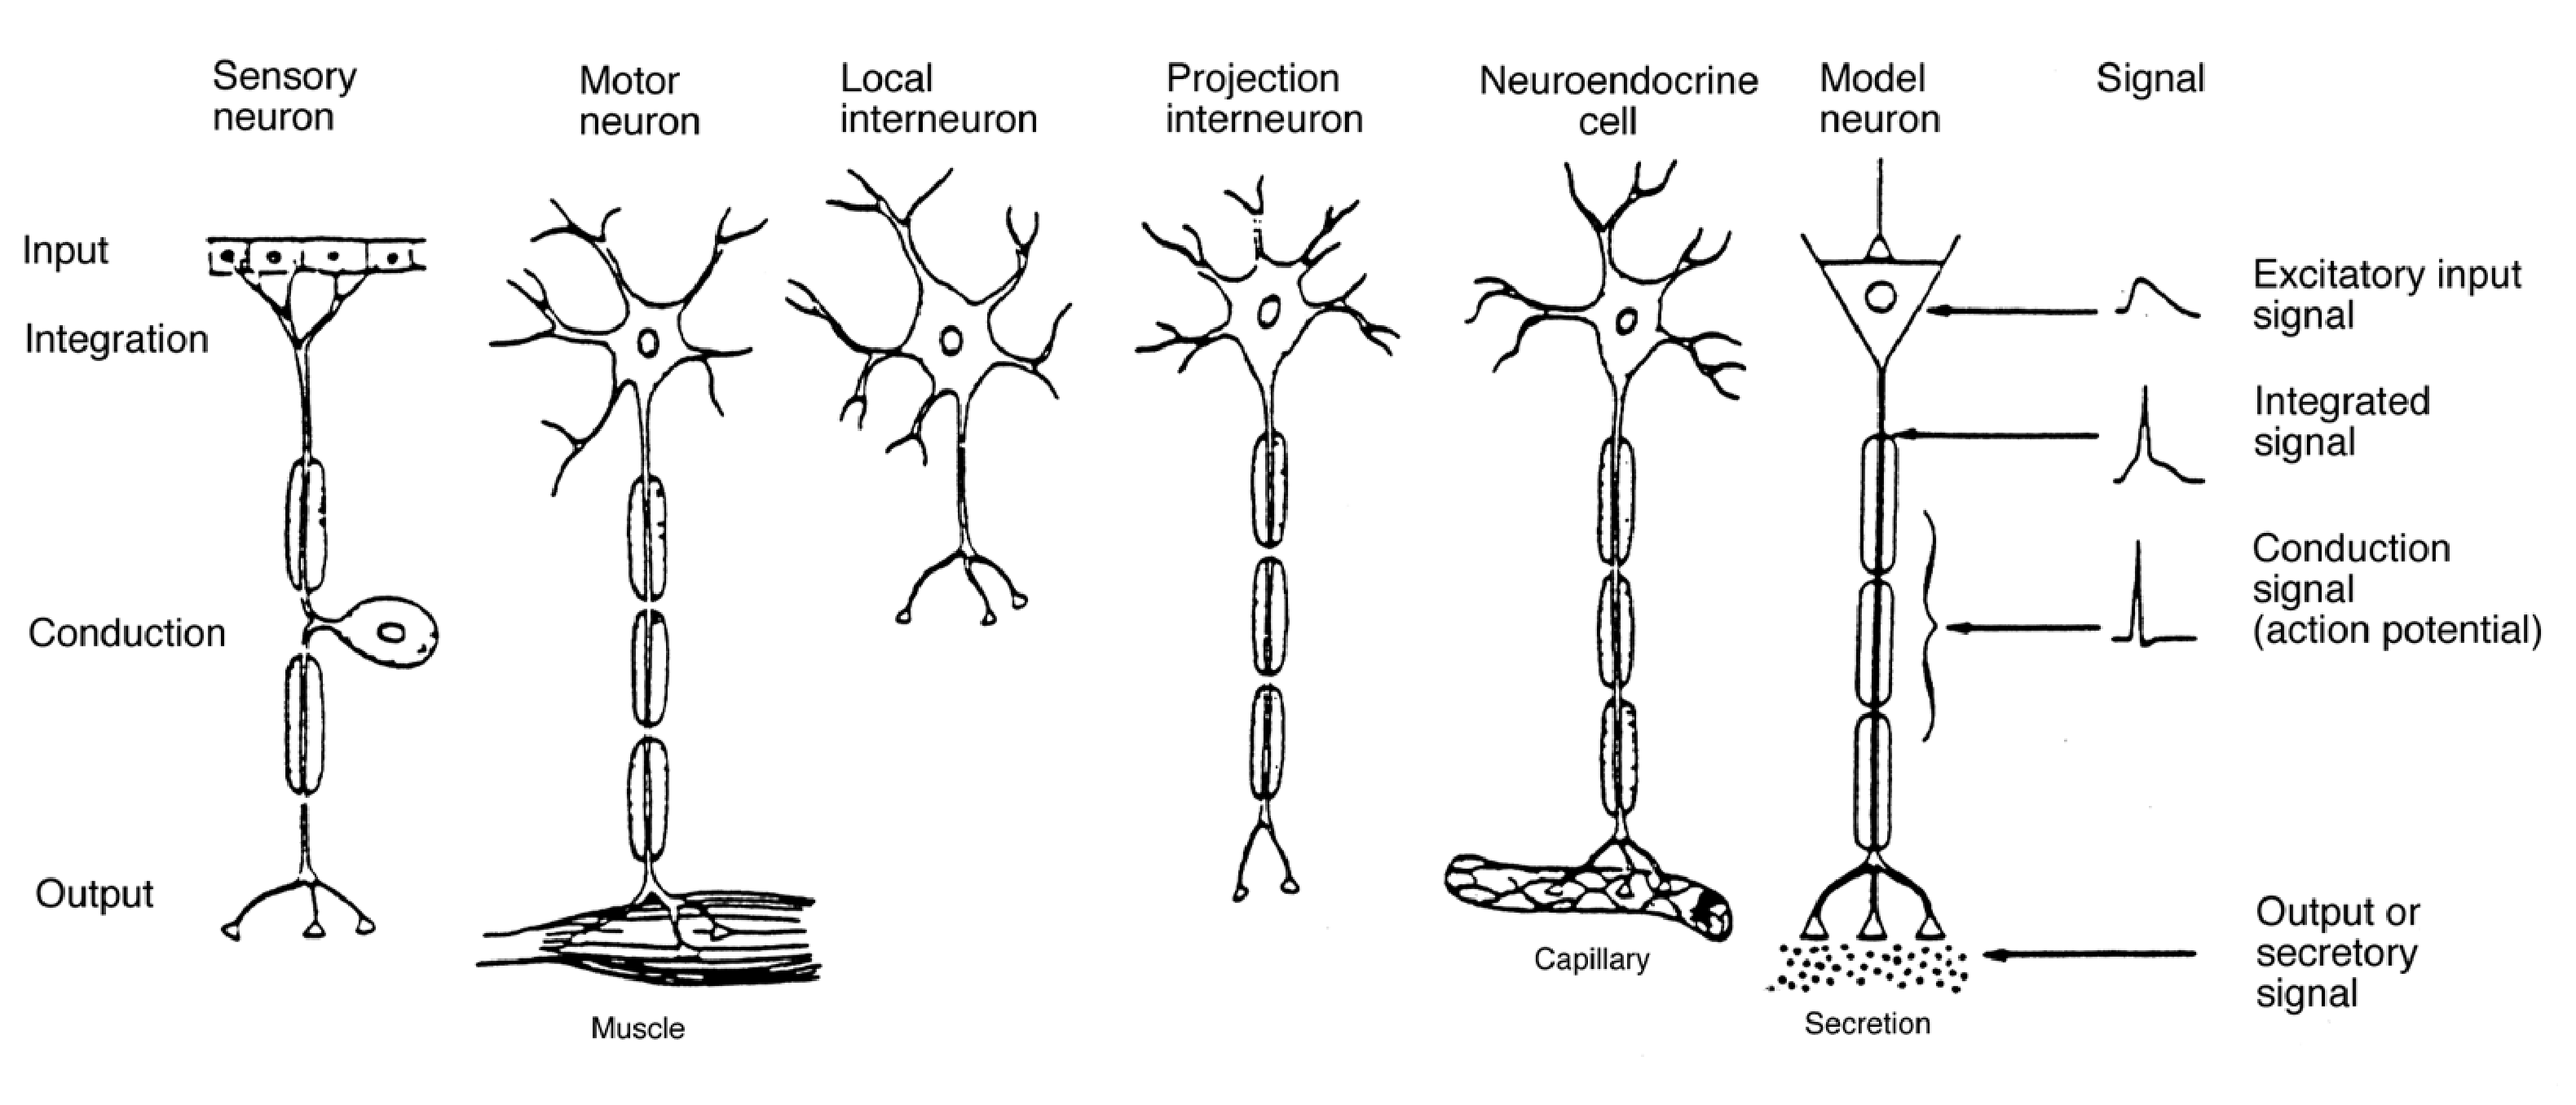
\includegraphics[width=\textwidth]{figures/bio_neurons}
	\caption{Examples of biological neurons}
\end{figure}
In the central nervous system, the nerve cells are supported by glia and blood vessels;
in the peripheral nervous system, they are supported by satellite cells, fibroblasts,
Schwann cells, and blood vessels.
There are three basic categories of neurons:
\begin{itemize}
	\item receptors : the ganglia of the spinal dorsal roots and of the cranial nerves
		with general sensory components,
	\item effectors : the ventral horn cells, motor cranial nerve nuclei, and motor division of
		the autonomic nervous system
	\item Interneurons, the vast majority of the neurons in the central nervous system.
\end{itemize}
The areas in the central nervous system that contain high numbers of neuronal cell bodies are
called gray matter, while the regions that contain primarily myelinated axons are called
white matter. Neurons are organized into ganglia, nuclei, or layered cortices.

There are two basic types of synapses, electrical and chemical, and they differ in location and 
appearance. Electrical synapses are connected by membrane bridges, gap junction and connections,
which permit the electric impulse to pass directly from one cell to the other.
Electric synapses have almost no delay and little chance of misfiring. These synapses are seen in 
many fish.Chemical synapses have a presynaptic side containing vesicles and a gap,
and a postsynaptic side with membrane receptors.
The neurotransmitter released by the action potential is exocytosed and diffuses across the 
synaptic cleft and binds to the specific receptor on the postsynaptic membrane.
Most of the synapses seen in the mammalian central nervous system are chemical.

If the voltage changes by a large enough amount over a short interval, 
the neuron generates an all-or-nothing electrochemical pulse called an action potential. 
This potential travels rapidly along the axon, and activates synaptic connections as it 
reaches them. Synaptic signals may be excitatory or inhibitory, 
increasing or reducing the net voltage that reaches the soma.
\begin{figure}[htb] 
	\label{fig:bio_activation}
	\centering
	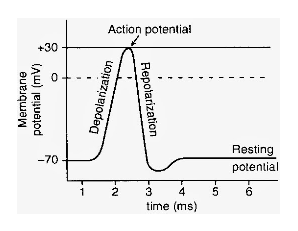
\includegraphics[width=0.6\textwidth]{figures/bio_activation}
	\caption{Examples of biological neurons}
\end{figure}
Chemical synapses consist of presynaptic axon terminals harboring synaptic vesicles and a
postsynaptic region (usually on dendrites) containing neurotransmitter receptors.
These neurotransmitters are made by the presynaptic neuron and stored in synaptic vesicles at
presynaptic terminals.
Whether a synapse is excitatory or inhibitory determines the postsynaptic current displayed,
which in turn is a function of the type of receptors and neurotransmitters operating at the
synapse
\begin{itemize}
	\item Excitatory synapses that  depolarize the membrane potential and make it more positive
		and they appear asymmetrical, having a prominent postsynaptic bush with presynaptic
		vesicles (Figs. 2.13 and 2.14 ). This type of synapse is most commonly seen on dendrites. 
		Glutamate has been identifi ed in excitatory synapses. At the excitatory synapse there is
		a change in permeability that leads to depolarization of the postsynaptic membrane and
		which can lead to the generation of an action potential.
	\item Inhibitory synapses thathyperpolarize the membrane potential and make it more negative.
		They are symmetrical with thickened membranes on the pre and postsynaptic side and
		vesicles only on the presynaptic side.
		GABA has been identifi ed in the inhibitory synapses. At an inhibitory synapse the
		neurotransmitter binds to the receptor membrane, which changes the permeability and tends
		to block the formation of the action potential. Synapses on the soma are symmetrical and 
		they are considered inhibitory.
	\item  Dendritic spines that are small membranous protrusions that contain the postsynaptic 
		machinery, including glutamate receptors, the actin cytoskeleton, and a wide variety of
		membrane-bound organelles, such as smooth endoplasmic reticulum, mitochondria, 
		and endosomes.
\end{itemize}
	

In this section the neuron model described by Lewis in 1968 (Lewis, 1968) is briefly discussed.
The Lewis model is based on the Hodgkin-Huxley membrane model and the theories of Eccles on 
synaptic transmission (Eccles, 1964). 
The model circuit is illustrated in Figure \ref{fig:lewis_neuron}.
This neuron model is divided into two sections: the synaptic section and the section generating
the action pulse.
Both sections consist of parallel circuits connected to the nodes representing the intracellular 
and extracellular sites of the membrane.
The section representing the synaptic junction is divided into two components. 
One of these represents the inhibitory junction and the other the excitatory junction. 
The sensitivity of the section generating the action pulse to a stimulus introduced at
the excitatory synaptic junction is reduced by the voltage introduced at the inhibitory junction.
The section generating the action pulse is based on the Hodgkin-Huxley model.
As described earlier, it consists of the normal circuits simulating the sodium and potassium 
conductances, the leakage conductance, and the membrane capacitance.
The circuit also includes an amplifier for the output signal.
This neuron model which is relatively complicated, is to be used in research on neural networks.
However, it is actually a simplified version of Lewis's 46-transistor network having the same form.
The purpose of this simplified Lewis model is to simulate the form of the action pulse, not with
the highest possible accuracy but, rather, with a sufficient accuracy provided by a simple model.
Figures 10.10, 10.11, and 10.12 show the behavior of the model compared to the simulation based 
directly on the Hodgkin and Huxley model.
From Figure 10.10 we find that when the stimulation current begins, the sodium ion current 
determined by Lewis (I'Na) rises to its peak value almost immediately, whereas the sodium ion
current of the Hodgkin-Huxley biological nerve (INa) rises much more slowly. 
The exponential decay of the current occurs at about the same speed in both. The behavior of the
potassium ion current is very similar in both the model and the biological membrane as simulated 
by Hodgkin and Huxley. 

\begin{figure}[htb] 
	\label{fig:lewis_neuron}
	\centering
	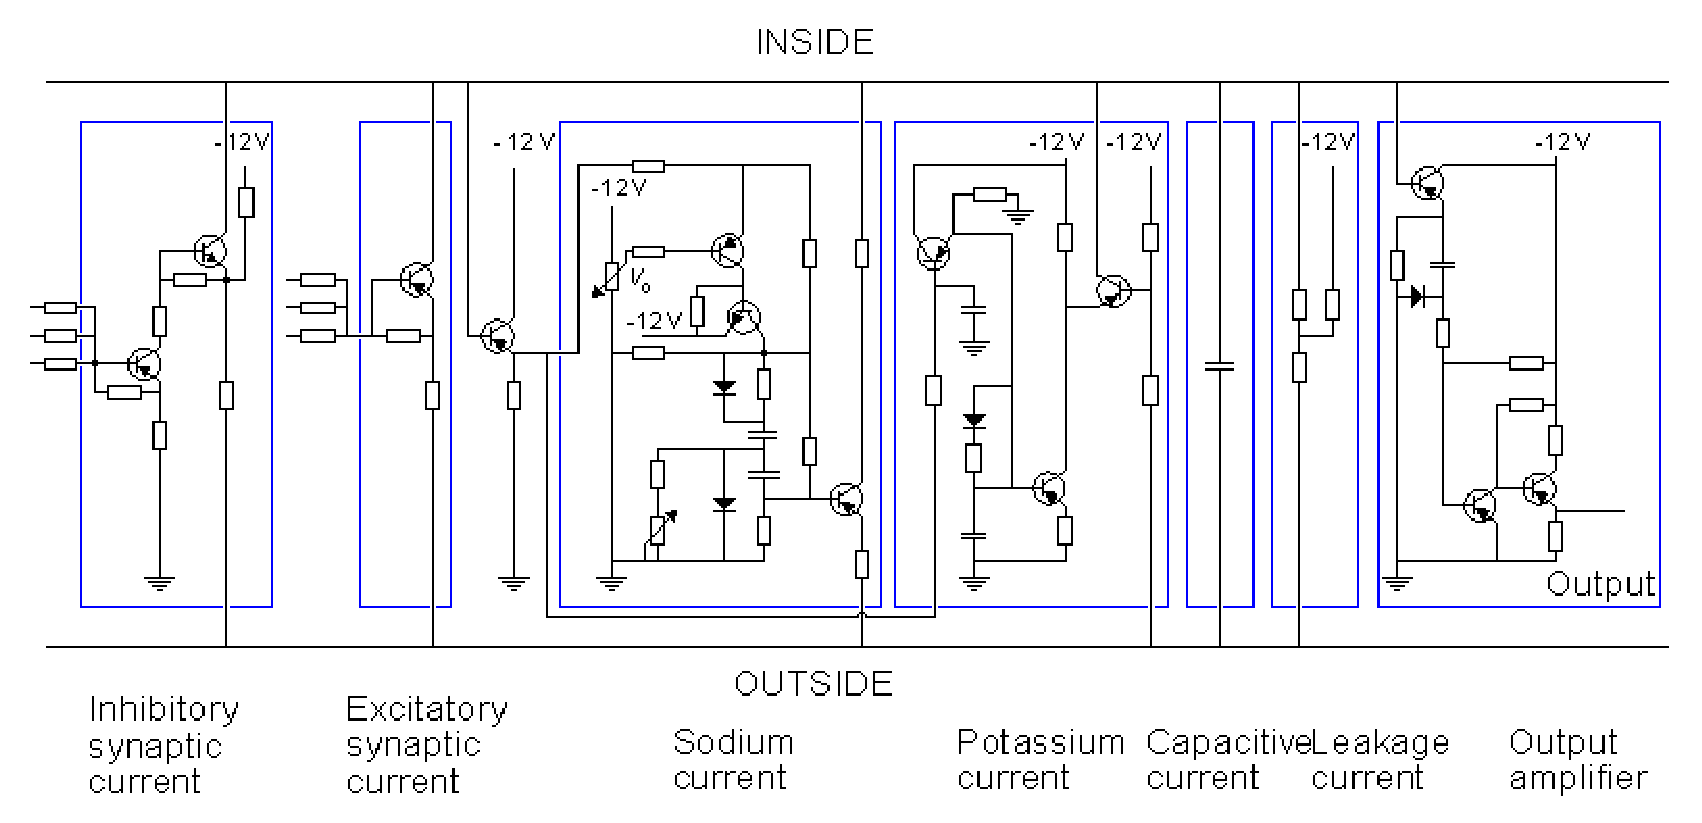
\includegraphics[width=0.8\textwidth]{figures/lewis_neuron}
	\caption{The Lewis neuron model from 1968.}
\end{figure}


The electronic realizations of the Hodgkin-Huxley model are very accurate in simulating the
function of a single neuron. However, when one is trying to simulate the function of neural 
networks, they become very complicated. 
Many scientists feel that when simulating large neural networks, the internal construction of 
its element may not be too important. It may be satisfactory simply to ensure that the elements 
produce an action pulse in response to the stimuli in a manner similar to an actual neuron. 
On this basis, Leon D. Harmon constructed a neuron model having a very simple circuit.
With this model he performed experiments in which he simulated many functions characteristic of
the neuron.
The circuit of the Harmon neuron model is given in Figure \ref{fig:harmon}.
The model is equipped with five excitatory inputs which can be adjusted. 
These include diode circuits representing various synaptic functions. 
The signal introduced at excitatory inputs charges the 0.02 $\mu F$ capacitor which, after reaching
a voltage of about 1.5 V, allows the monostable multivibrator, formed by transistors T1 and T2, 
to generate the action pulse. This impulse is amplified by transistors T3 and T4. 
The output of one neuron model may drive the inputs of perhaps 100 neighboring neuron models.
The basic model also includes an inhibitory input. A pulse introduced at this input has the effect
of decreasing the sensitivity to the excitatory inputs.. 
\begin{figure}[htb] 
	\label{fig:harmon}
	\centering
	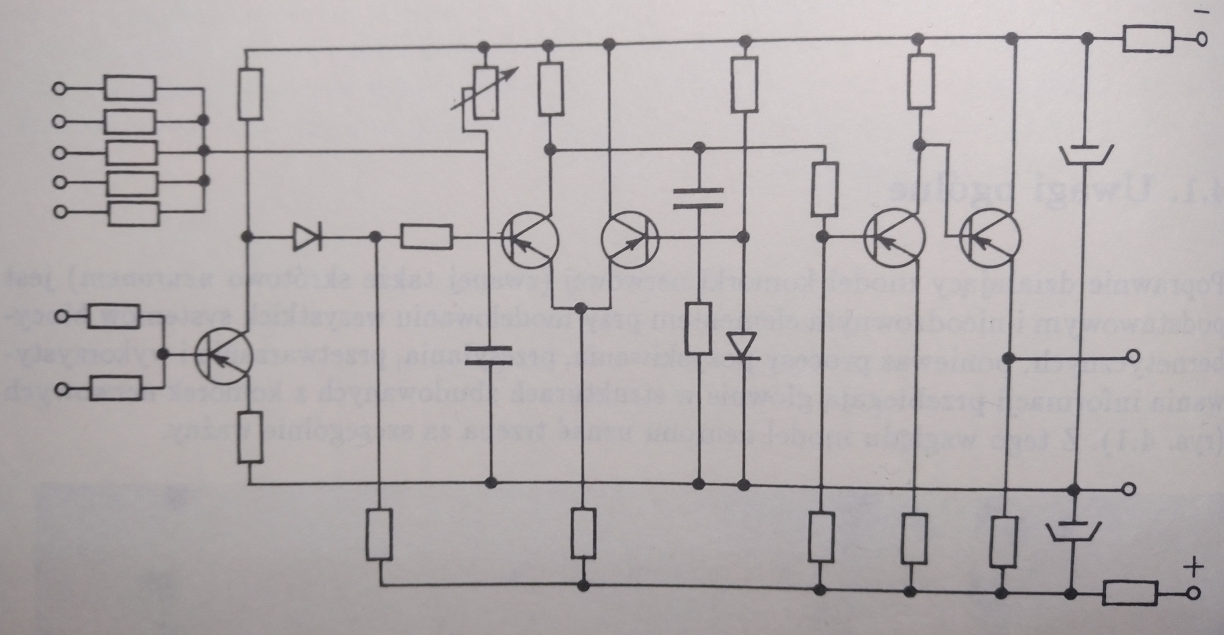
\includegraphics[width=0.8\textwidth]{figures/harmon}
	\caption{Harmon electrical model of neurall cell}
\end{figure}
%----------------------------------------------------------------------------------------------------
\subsection{Artificial representation of biological neuron}
\FloatBarrier
In 1943 Warren S. McCulloch, a neuroscientist, and Walter Pitts, a logician, 
published "A logical calculus of the ideas immanent in nervous activity" in the 
Bulletin of Mathematical Biophysics 5:115-133. In this paper McCulloch and Pitts tried to
understand how the brain could produce highly complex patterns by using many basic cells
that are connected together. 
McCulloch Pitts neuron is a highly simplified model of neural cell that models only a most
basic behavior of electrical signal transmition.
Neuron is divided into three blocks:
\begin{enumerate}
	\item aggregation where many input signals $\{x_{1}, x_{2}, \cdots, x_{n}\}$ are 
		aggregated into single signal $\hat{u}$,
	\item dampening where signal strength is reduced according to bias term and dampened 
		response $u$ is returned,
	\item activation where signal $u$ is transformed to neuron response space.
\end{enumerate}
Response of neuron modelled like that can be written as:
\begin{equation}
	\label{equ:neuron_response}
	h_{x} = f_{a}(u(\hat{u}(x))),
\end{equation}
however as in most cases weighted sum is realisation of aggregation and dampening is handled by
a simple substation neuron equation is simplified to: 
\begin{equation}
	\label{equ:neuron_response}
	h_{x} = f_{a}(u(x)).
\end{equation}
In case of McCulloch Pitts neuron both aggregation and dampening are realised by a single 
linear function akin to linear predictor:
\begin{equation}
	\label{equ:linear_neuron}
	u(x) = \Theta_{0} + \Theta_{1}x_{1} + \cdots + \Theta_{n}x_{n},
\end{equation}
which as described in chapter \ref{sec:linear_regression} can be written in a matrix notation as
\begin{equation}
	\label{equ:linear_neuron_matrix}
	u(X) = \Theta^{T}\cdot X.
\end{equation}
Almost all modern implementations of artificial neural networks use this aggregation, dampening
model and the only difference between them is in an activation function.
McCulloch Pitts neuron uses step function as an activation:
\[
	\label{equ:step_function}
	 f_{STEP}(u)=
	\begin{cases}
		1,&  u > 0, \\
		0,&  u \leq 0,
	\end{cases}
	.
\]
With this function neuron can process signals however it still lacks a very important function
of a biological neuron, ability to learn. First learning algorithm developed on base of 
McCulloch Pitts neuron was perceptron algorithm created by \textbf{TODO: BY WHO}.
With $\hat{y}$ defined as a neuron prediction and $y$ as a expected output perceptron learning
algorithm can me described as:
\begin{enumerate}
	\item if $\hat{y}=y$ then do nothing,
	\item if $\hat{y}=1$ and $y=0$ then $\Theta \leftarrow \Theta + x$
	\item if $\hat{y}=0$ and $y=1$ then $\Theta \leftarrow \Theta - x$
\end{enumerate}
Due to its ability to separate space into two subspaces perceptron can be used to model a logical
operators and as such realise logical reasoning.
Let's start with the AND operator.  Looking back at the logic table for the $A\land B$, 
we can see that we only want the neuron to output a 1 when both inputs are activated.
To do this, we want the sum of both inputs to be greater than the threshold, but each input alone
must be lower than the threshold.  Let's use a threshold of 1. 
So, now we need to choose the weights according to the constraints I've just explained - 
how about 0.6 and 0.6?  With these weights, individual activation of either input A or B will 
not exceed the threshold, while the sum of the two will be 1.2, which exceeds the threshold 
and causes the neuron to fire.
I've used a greek letter theta to denote the threshold, which is quite common practice. 
A and B are the two inputs.  You can think of them as input neurons, like photoreceptors, 
taste buds, olfactory receptors, etc.  They will each be set to 1 or 0 depending upon the truth of
their proposition.  The red neuron is our decision neuron. 
If the sum of the synapse-weighted inputs is greater than the threshold, 
this will output a 1, otherwise it will output a 0.  
So, to test it by hand, we can try setting A and B to the different values in the 
truth table and seeing if the decision neuron's output matches the $A\land B$ column:
\begin{itemize}
	\item  $A=0 \land B=0  \to   \hat{y} = 0*1  +  0*1 - 1  = -1 \to$,
	\item $A=0 \land B=1  \to  \hat(y) = 0*1  +  1*1  = 0.6$,
	\item $A=1 \land B=0  \to  \hat(y) = 1*1  +  0*1  = 0.6$,
	\item $A=1 \land B=1  \to  \hat(y) = 1*1  +  1*1  = 1.2$.
\end{itemize}

We have designed a neuron which implements a logical AND gate.  

This is easy to implement in Excel.  In fact, it's exactly the same as the neuron we 
created in What does a neuron do.  

Next up is the OR gate.  Look back at the logic table.  In this case, we want the output to 
be 1 when either or both of the inputs, A and B, are active, but 0 when both of the inputs are 0.  
This is simple enough.  If we make each synapse greater than the threshold, 
then it'll fire whenever there is any activity in either or both of A and B.
This is shown on the right.  Synaptic values of 1.1 are sufficient to surpass 
the threshold of 1 whenever their respective input is active.  
	

%----------------------------------------------------------------------------------------------------
\subsection{Feed forward neural networks}
\FloatBarrier

\begin{figure}[htb] 
	\label{fig:xor_gates}
	\centering
	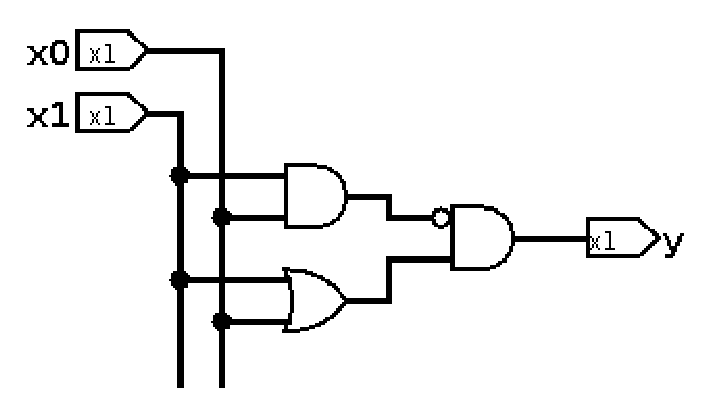
\includegraphics[width=0.6\textwidth]{figures/xor_gates}
	\caption{Implementation of XOR gate with AND, OR and NOT gates}
\end{figure}

\begin{figure}[htb] 
	\label{fig:neuro_xor}
	\centering
	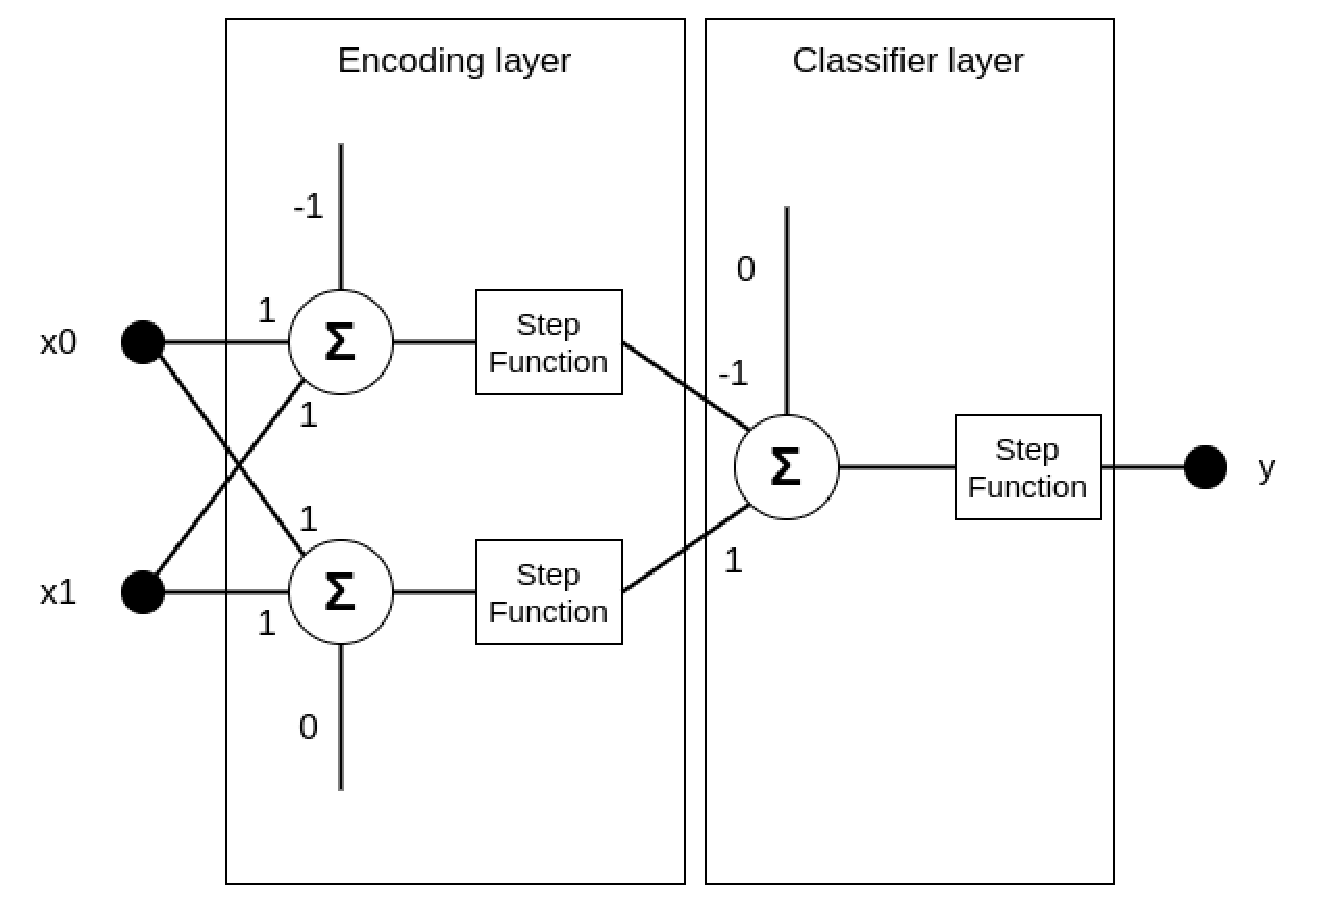
\includegraphics[width=\textwidth]{figures/neuro_xor}
	\caption{Neuron based equivalent of XOR function}
\end{figure}

%----------------------------------------------------------------------------------------------------
\subsection{Simple recurrent neural networks}
Simple solution to problem of time independence is to concatenate response of neural layer
from previous cycle to it input 
\begin{equation}
	\label{equ:sru_input}
	x'(t)=[x(t)|y(t-1)]
\end{equation}
Such solution results in signal propagating trough time and influencing responses of future cycles,
if this is only modification to feed forward model such layer is called simple recurrent
unit (SRU).
While this solution makes model time aware it have its own problems, mainly a signal vanishing
issue. Since the input signal from cycle $n$ have direct influence only on a response of this
cycle and for each subsequent cycles it is only trough feedback loop. Influence of input $n$ on
response of cycle $n+k$ grows inverse proportional to $k$.
This means that in this model only those regularities that appear over short time periods can
be detected.
Making weights on feedback bigger will not eliminate problem and instead replace it with signal
explosion that causes response to reach maximum value if a strong signal appeared on input at
least once.

%----------------------------------------------------------------------------------------------------
\subsection{Networks with long term memory}
\FloatBarrier
One of possible solutions to this issue is addition of long term memory which will regulate
forward and loop back path influence on neuron response, such solution is used in long short
term memory (LSTM) networks \cite{Hochreiter1997}.
\begin{figure}[htb] 
	\label{fig:lstm}
	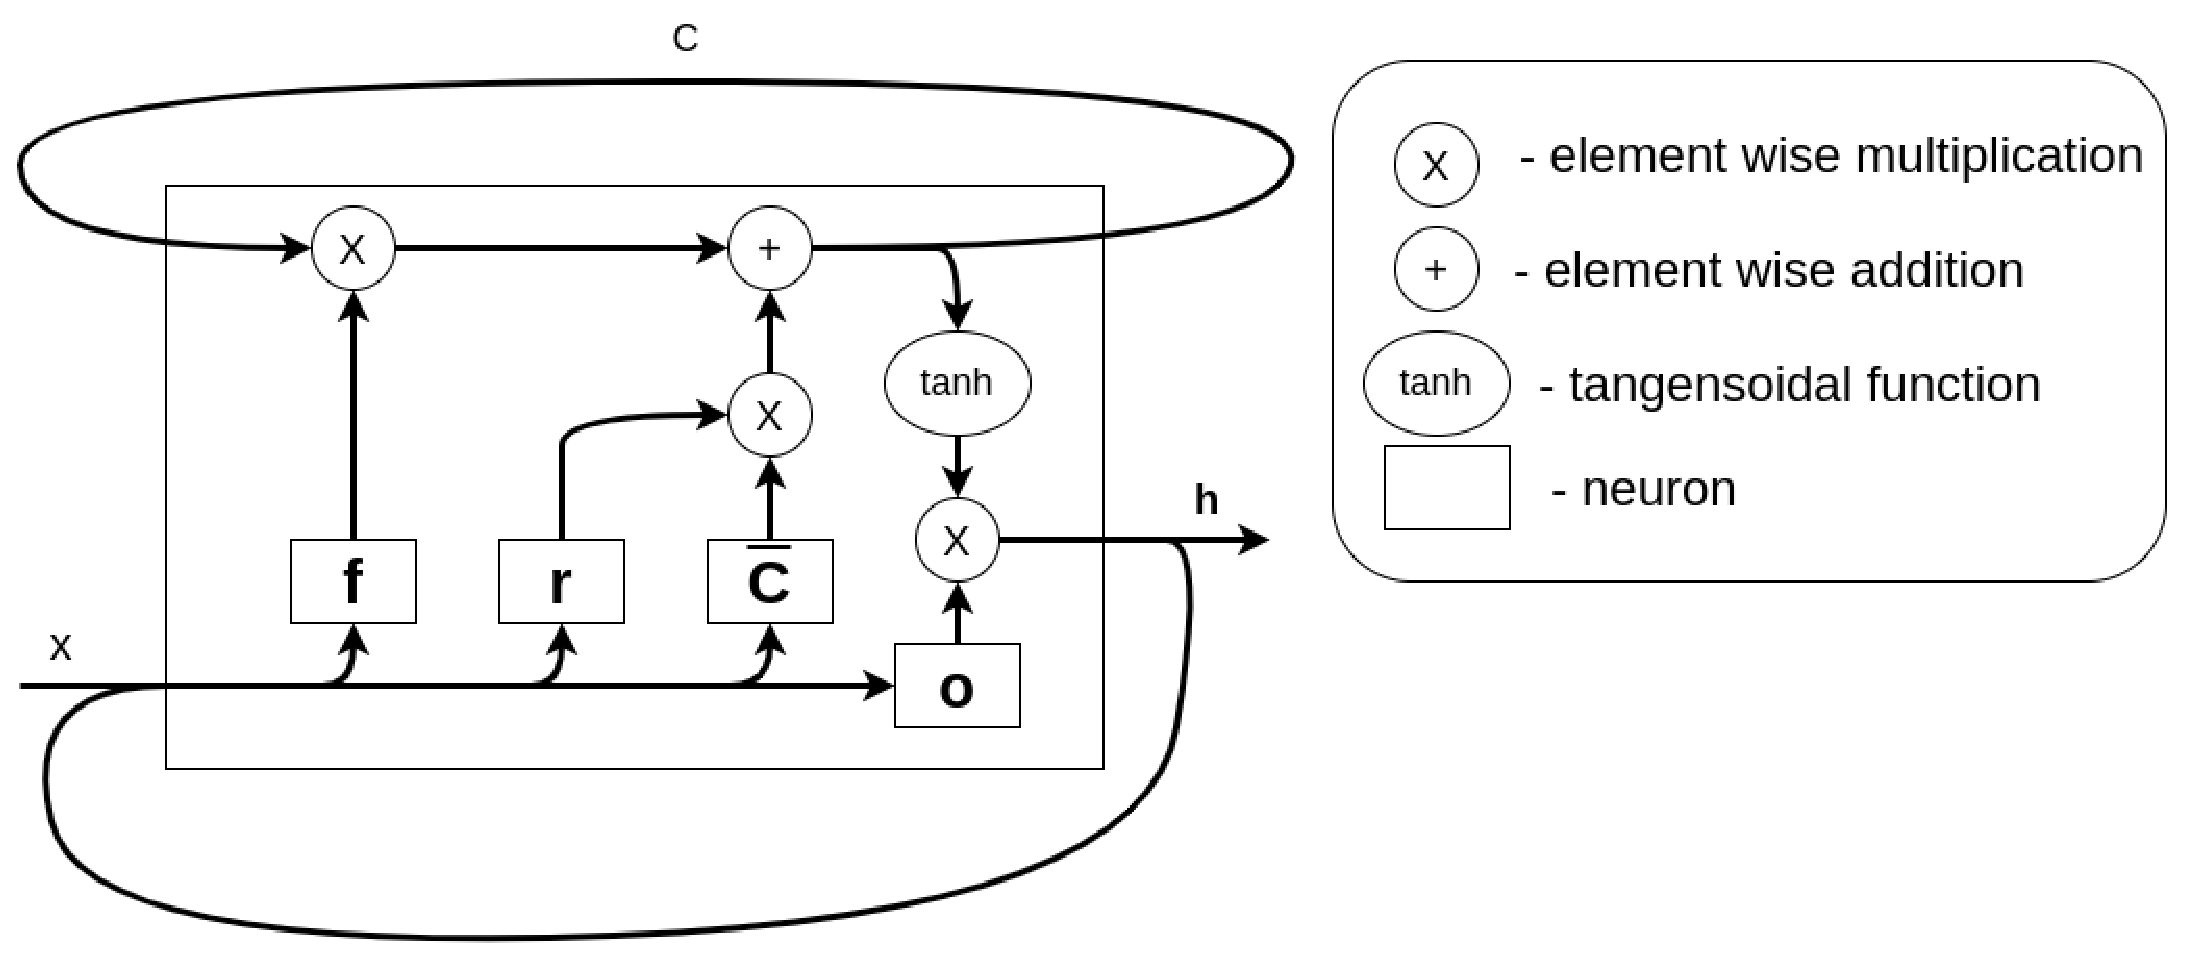
\includegraphics[width=\textwidth]{figures/lstm}
	\caption{LSTM layer}
\end{figure}
Single LSTM neuron consists of 4 basic neurons and two non neuron operations:
\begin{itemize}
\item $x'(t)=[x(t)|y(t-1)]$,
\item $o_t=\sigma (W_o\cdot x'_t+b_o)$,
\item $r_t=\sigma (W_r\cdot x'_t+b_r)$,
\item $f_t=\sigma (W_f\cdot x'_t+b_f)$,
\item $\bar{C}_t=\tanh (W_c\cdot x'_t+b_c)$,
\item $C_t=f_t\circ C_{t-1}+r_t\circ \bar{C}_t$,
\item $y_t=o_t\circ \tanh (C_t)$.
\end{itemize}
With $W$ and $b$ being weights and biases for each basic neuron, $x$ input, $y$ output and
$C$ long term memory. As it can be seen $o_t$ is a equivalent of SRU and is moderated by
long term memory before propagating as output. Temporary value of long term memory based
only on current output $\bar{C}_t$ is calculated and then with help of neurons $r$ and $f$
is transformed into its final value.
Neuron $r$ is called remembering gate and influences to what degree temporary long term
memory from given cycle effects its final value while $f$ is forgetting gate and
decides influence of long term memory from last cycle on current one.
Thanks to such implementation model can learn to detect long term regularities as well
as short term ones.
Gated recurrent units (GRUs) are a gating mechanism in recurrent neural networks,
introduced in 2014 by Kyunghyun Cho et al.
The GRU is like a long short-term memory (LSTM) with a forget gate, but has fewer parameters 
than LSTM, as it lacks an output gate. GRU's performance on certain tasks of polyphonic music
modeling, speech signal modeling and natural language processing was found to be similar 
to that of LSTM. GRUs have been shown to exhibit better performance on certain smaller and less
frequent datasets.
\begin{figure}[htb] 
	\label{fig:gru}
	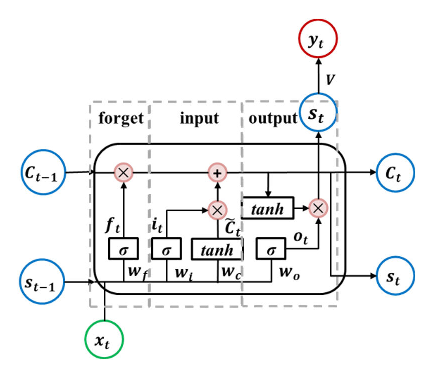
\includegraphics[width=0.7\textwidth]{figures/gru}
	\caption{GRU layer}
\end{figure}
The minimal gated unit is similar to the fully gated unit, except the update and reset gate vector
is merged into a forget gate. This also implies that the equation for the output vector 
must be changed.

%----------------------------------------------------------------------------------------------------
\subsection{Backpropagation Through Time}
\FloatBarrier
Backpropagation Through Time (BPTT) is the algorithm that is used to update the weights in the 
recurrent neural network. 
One of the common examples of a recurrent neural network is LSTM. 
Backpropagation is an essential skill that you should know if you want to effectively frame 
sequence prediction problems for the recurrent neural network. You should also be aware of the
effects of the Backpropagation Through time on the stability, the speed of the system while 
training the system.
The ultimate goal of the Backpropagation algorithm is to minimize the error of the network outputs.

The Backpropagation Through Time is the application of Backpropagation training algorithm which 
is applied to the sequence data like the time series. It is applied to the 
recurrent neural network. 
The recurrent neural network is shown one input each timestep and predicts the corresponding
output. So, we can say that BTPP works by unrolling all input timesteps.
Each timestep has one input time step, one output time step and one copy of the network.
Then the errors are calculated and accumulated for each timestep.
The network is then rolled back to update the weights.
But one of the disadvantages of BPTT is when the number of time steps increases the computation
also increases. This will make the overall model noisy. The high cost of single parameter updates
makes the BPTT impossible to use for a large number of iterations.
This is where Truncated Backpropagation comes save the day for us. 
Truncated Backpropagation (TBPTT) is nothing but a slightly modified version of BPTT algorithm 
for the recurrent neural network. In this, the sequence is processed one timestep at a time and
periodically the BPTT update is performed for a fixed number of time steps.

The basic Truncated Backpropagation algorithm is
\begin{enumerate}
    \item First, give the sequence of, say K1 time steps of input and output pairs to the network.
    \item Then calculate and accumulate the errors across say, k2 time steps 
		by unrolling the network
    \item Finally, update the weights by rolling up the network
\end{enumerate}
As you can clearly see that you need two parameters namely k1 and k2 for implementing TBPTT. 
K1 is the number of forwarding pass timesteps between updates.
This influences how fast or slow will be the training and the frequency of the weight updates. 
On the other hand, k2 is the number of timesteps which apply to BPTT. 
It should be large enough to capture the temporal structure in the problem 
for the network to learn. 

%====================================================================================================
\section{Overfitting}
\FloatBarrier
Overfitting is a concept in data science, which occurs when a statistical model fits exactly
against its training data. 
When this happens, the algorithm unfortunately cannot perform accurately against unseen data,
defeating its purpose.
Generalization of a model to new data is ultimately what allows us to use machine learning
algorithms every day to make predictions and classify data.
When machine learning algorithms are constructed, they leverage a sample dataset 
to train the model. 
However, when the model trains for too long on sample data or when the model is too complex, 
it can start to learn the “noise,” or irrelevant information, within the dataset. 
When the model memorizes the noise and fits too closely to the training set, 
the model becomes “overfitted,” and it is unable to generalize well to new data.
If a model cannot generalize well to new data, then it will not be able to perform the
classification or prediction tasks that it was intended for.

Low error rates and a high variance are good indicators of overfitting.
In order to prevent this type of behavior, part of the training dataset is typically set aside 
as the “test set” to check for overfitting. 
If the training data has a low error rate and the test data has a high error rate, 
it signals overfitting.

%----------------------------------------------------------------------------------------------------
\subsection{Early stoppingi}
\FloatBarrier
Regularization by early stopping can be done either by dividing the dataset into training and test 
sets and then using cross-validation on the training set or by dividing the dataset into training, 
validation and test sets, in which case cross-validation is not required.
Here, the second case is analyzed. In early stopping, the algorithm is trained using the
training set and the point at which to stop training is determined from the validation set. 
Training error and validation error are analysed. The training error steadily decreases while 
validation error decreases until a point, after which it increases. 
This is because, during training, the learning model starts to overfit to the training data. 
This causes the training error to decrease while the validation error increases.
So a model with better validation set error can be obtained if the parameters that give the least
validation set error are used.
Each time the error on the validation set decreases, a copy of the model parameters is stored.
When the training algorithm terminates, these parameters which give the least validation set
error are finally returned and not the last modified parameters. 
\begin{figure}[htb] 
	\label{fig:early_stop}
	\centering
	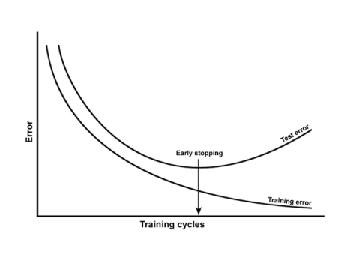
\includegraphics[width=0.6\textwidth]{figures/early_stop}
	\caption{Neuron based equivalent of XOR function}
\end{figure}

In Regularization by Early Stopping, we stop training the model when the performance of the 
model on the validation set is getting worse-increasing loss or decreasing accuracy or poorer 
values of the scoring metric. By plotting the error on the training dataset and the validation 
dataset together, both the errors decrease with a number of iterations until the point where 
the model starts to overfit.
After this point, the training error still decreases but the validation error increases. 
So, even if training is continued after this point, early stopping essentially returns the set of
parameters which were used at this point and so is equivalent to stopping training at that point.
So, the final parameters returned will enable the model to have low variance and 
better generalization. 
The model at the time the training is stopped will have a better generalization performance than
the model with the least training error. 
Early stopping can be thought of as implicit regularization, contrary to regularization via 
weight decay. 
This method is also efficient since it requires less amount of training data,
which is not always available. Due to this fact, early stopping requires lesser time for training 
compared to other regularization methods. 
Repeating the early stopping process many times may result in the model overfitting the
validation dataset, just as similar as overfitting occurs in the case of training data.

The number of iterations taken to train the model can be considered as a hyperparameter.
Then the model has to find an optimum value for this hyperparameter(by hyperparameter 
tuning)for the best performance of the learning model.


%----------------------------------------------------------------------------------------------------
\subsection{$\ell$ regularization}
\FloatBarrier
A regression model that uses L1 regularization technique is called Lasso Regression and model i
which uses L2 is called Ridge Regression.
The key difference between these two is the penalty term.

Ridge regression adds ``squared magnitude'' of coefficient as penalty term to the loss function.
Here the highlighted part represents L2 regularization element.
\begin{equation}
	\label{equ:ridge_regression}
	\sum_{i=1}^{n}(y_{i}-\sum_{j=1}^{p}x_{ij}\beta_{j})^{2} + \lambda \sum_{j=1}^{p}\beta_{j}^{2},
\end{equation}
Here, if lambda is zero then you can imagine we get back OLS.
However, if lambda is very large then it will add too much weight and it will lead to
under-fitting. Having said that it’s important how lambda is chosen.
This technique works very well to avoid over-fitting issue.

Lasso Regression (Least Absolute Shrinkage and Selection Operator) adds
``absolute value of magnitude'' of coefficient as penalty term to the loss function.
\begin{equation}
	\label{equ:lasso_regresson}
	\sum_{i=1}^{n}(Y_{i}-\sum_{j=1}^{p}X_{ij}\beta_{j})^{2} + \lambda \sum_{j=1}^{p}
	\vert \beta_{j} \vert,
\end{equation}
Again, if lambda is zero then we will get back OLS whereas very large value will make coefficients 
zero hence it will under-fit.
The key difference between these techniques is that Lasso shrinks the less important feature’s 
coefficient to zero thus, removing some feature altogether. 
So, this works well for feature selection in case we have a huge number of features.

%----------------------------------------------------------------------------------------------------
\subsection{Dropout}
\FloatBarrier
Deep neural networks contain multiple non-linear hidden layers and this makes them very
expressive models that can learn very complicated relationships between their inputs and
outputs. With limited training data, however, many of these complicated relationships
will be the result of sampling noise, so they will exist in the training set but not in real
test data even if it is drawn from the same distribution. This leads to overfitting and many
methods have been developed for reducing it. These include stopping the training as soon as
performance on a validation set starts to get worse, introducing weight penalties of various
kinds such as L1 and L2 regularization and soft weight sharing (Nowlan and Hinton, 1992).

With unlimited computation, the best way to “regularize” a fixed-sized model is to
average the predictions of all possible settings of the parameters, weighting each setting by
its posterior probability given the training data. This can sometimes be approximated quite
well for simple or small models (Xiong et al., 2011; Salakhutdinov and Mnih, 2008), but we
would like to approach the performance of the Bayesian gold standard using considerably
less computation. We propose to do this by approximating an equally weighted geometric
mean of the predictions of an exponential number of learned models that share parameters.
Model combination nearly always improves the performance of machine learning meth-
ods. With large neural networks, however, the obvious idea of averaging the outputs of
many separately trained nets is prohibitively expensive. Combining several models is most
helpful when the individual models are different from each other and in order to make
neural net models different, they should either have different architectures or be trained
on different data. Training many different architectures is hard because finding optimal
hyperparameters for each architecture is a daunting task and training each large network
requires a lot of computation. Moreover, large networks normally require large amounts of
training data and there may not be enough data available to train different networks on
different subsets of the data. Even if one was able to train many different large networks,
using them all at test time is infeasible in applications where it is important to respond
quickly.
Dropout is a technique that addresses both these issues. It prevents overfitting and
provides a way of approximately combining exponentially many different neural network
architectures efficiently. The term “dropout” refers to dropping out units (hidden and
visible) in a neural network. By dropping a unit out, we mean temporarily removing it from
the network, along with all its incoming and outgoing connections, as shown in Figure 1.
The choice of which units to drop is random. In the simplest case, each unit is retained with
a fixed probability p independent of other units, where p can be chosen using a validation
set or can simply be set at 0.5, which seems to be close to optimal for a wide range of
networks and tasks. For the input units, however, the optimal probability of retention is
usually closer to 1 than to 0.5.
\begin{figure}[htb] 
	\label{fig:dropout}
	\centering
	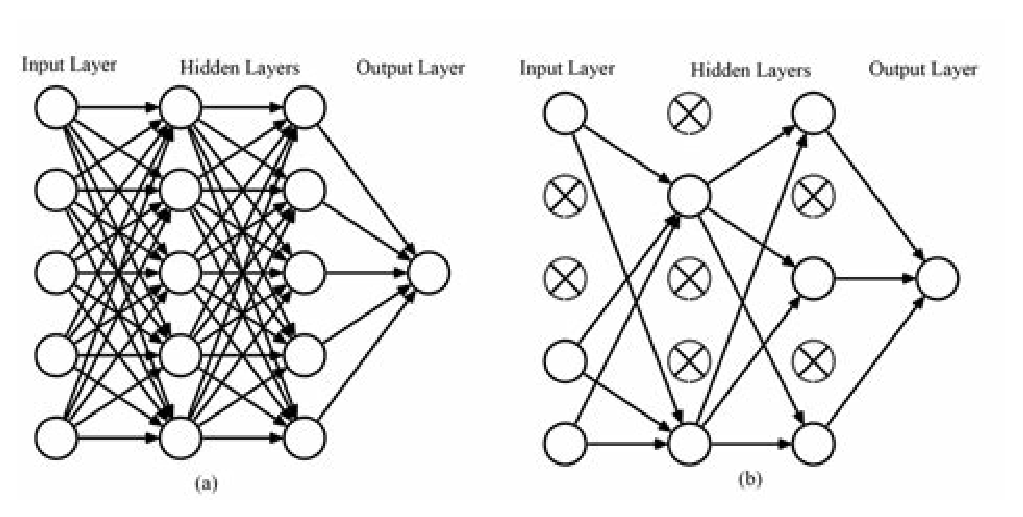
\includegraphics[width=\textwidth]{figures/dropout}
	\caption{Dropout Neural Net Model. Left: A standard neural net with 2 hidden layers.
	Right: An example of a thinned net produced by applying dropout to the network on the left.
	Crossed units have been dropped}
\end{figure}

Applying dropout to a neural network amounts to sampling a “thinned” network from
it. The thinned network consists of all the units that survived dropout (Figure 1b). A
neural net with n units, can be seen as a collection of 2 n possible thinned neural networks.
These networks all share weights so that the total number of parameters is still O(n 2 ), or
less. For each presentation of each training case, a new thinned network is sampled and
trained. So training a neural network with dropout can be seen as training a collection of 2 n
thinned networks with extensive weight sharing, where each thinned network gets trained
very rarely, if at all.
At test time, it is not feasible to explicitly average the predictions from exponentially
many thinned models. However, a very simple approximate averaging method works well in
practice. The idea is to use a single neural net at test time without dropout. The weights
of this network are scaled-down versions of the trained weights. If a unit is retained with
probability p during training, the outgoing weights of that unit are multiplied by p at test
time as shown in Figure 2. This ensures that for any hidden unit the expected output (under
the distribution used to drop units at training time) is the same as the actual output at
test time. By doing this scaling, 2 n networks with shared weights can be combined into
a single neural network to be used at test time. We found that training a network with
dropout and using this approximate averaging method at test time leads to significantly
lower generalization error on a wide variety of classification problems compared to training
with other regularization methods.
The idea of dropout is not limited to feed-forward neural nets. It can be more generally
applied to graphical models such as Boltzmann Machines. In this paper, we introduce
the dropout Restricted Boltzmann Machine model and compare it to standard Restricted
Boltzmann Machines (RBM). Our experiments show that dropout RBMs are better than
standard RBMs in certain respects.
This paper is structured as follows. Section 2 describes the motivation for this idea.
Section 3 describes relevant previous work. Section 4 formally describes the dropout model.
Section 5 gives an algorithm for training dropout networks. In Section 6, we present our
experimental results where we apply dropout to problems in different domains and compare
it with other forms of regularization and model combination. Section 7 analyzes the effect of
dropout on different properties of a neural network and describes how dropout interacts with
the network’s hyperparameters. Section 8 describes the Dropout RBM model. In Section 9
we explore the idea of marginalizing dropout. In Appendix A we present a practical guide
for training dropout nets. This includes a detailed analysis of the practic.
